\chapter{Data Analysis}
\label{ch:analysis}
The first production run at JLab's Hall B after the completion of the 12 GeV upgrade was called Run Group A. It ran over the fall of 2018 and spring 2019 with billions of events and 2 pB of data accumulated. The beam energy for the run was 10.6 GeV on a 5 cm liquid hydrogen target at a current between 5 nA to 75 nA. Because this is the first set of data coming from CLAS12 detectors, it serves as the data from which all important calibration and analysis is done to better understand all subsequent run groups.

This chapter will outline the software tools used for turning raw data into usable data sets, and the calibrations done to correct the raw data. Then we will begin the analysis portion, extracting the inclusive DIS cross section from Run Group A. Here we must make fiducial cuts to eliminate inefficient areas of individual detectors and kinematic cuts to select DIS events. Finally we put the resulting data together into bins of $x$ and $y$ (where $y=\nu/E$) to find the acceptance and calculate the inclusive DIS cross section. The purpose of extracting this cross section is to compare it the well-established Christy-Bosted fits to data.

\section{CLAS12 Offline Software}
The raw data coming from each detector first enters into the ReadOut Controller (ROC) and then gets stored in the EVent Input Output (EVIO) format. EVIO is a data format that is designed and maintained by JLab Data Acquisition Group. Once that data is available for off-line use, it requires decoding. Decoding is the process of taking EVIO raw data and converting it to High Output Performance Output (HIPO) format. 

The HIPO format provides for a flexible data container structure, and minimizes disk space by utilizing LZ4 data compression (the fastest compression method currently available). In each HIPO file, data is stored as individual records with adjustable size. Each record is compressed, with a tag associated with it, and a pointer to it is stored in the file's index table. For analysis this provides users with faster analysis by reading portions of the file depending on the final states to be analyzed.

Once the data is in HIPO format, it is ready to by reconstructed and analyzed. The CLAS12 event Reconstruction and Analysis (or CLARA) framework allows users to reconstruct physics events and analyze the files to yield usable physical data. CLARA does this by utilizing an service-oriented architecture to enhance agility, efficiency, and productivity of the software components within the CLARA framework. During the reconstruction process, the raw data from all detectors is taken in and processed by the corresponding packages. The main packages in CLARA are for \textit{geometry}, \textit{calibration constants}, \textit{magnetic fields}, \textit{particle swimming}, and \textit{plotting/analysis}.

The geometry tools were created due to the complexity of the CLAS12 subsystem geometries. The library contains primitives that represent all of the lines, planes and shapes of all the detectors. The tools provide methods to track particles through the different volumes for evaluation of track trajectories, such as line-to-surface intersections, ray tracing through objects, and evaluation of the distance of closest approach to a line or surface.  Because subsystem parameters can change from run group to run group and sometimes even within a run group, time-dependent geometry variations exist that allows for consistency between simulation, reconstruction, and event visualization packages.

The Calibration Constants Database (CCDB) was originally developed at JLab for the GlueX Experiment in Hall D. It was adopted by CLAS12 group because of its functionality for storing and accessing structured tables. At the decoding stage, file formats change, but also data structures. Signals are converted from hardware notation ($i.e.$ crate, slot, channel) to CLAS12 notation ($i.e.$ sector, layer, component). Then during reconstruction, the time stamps of these databases are utilized in order to access run-specific constants. The CLAS12 software tools employ an Application Programming Interface (API) that parses CCDB tables to create structured maps of the constants stored in memory by sector, layer, component. This method allows for fast retrieval of only the relevant constants.

\textit{Magfield}, the magnetic field package for CLARA, consists of binary field maps created from engineering models of the solenoid and torus magnets in CLAS12. These field maps contain a header with meta-data describing field pedigree, its grid coordinate system, and the coordinate system of the field components. Because the field is often accessed within a sequence of points all contained within a single grid, \textit{magfield} uses time-saving software probes to cache nearest neighbors.

To propagate charged particles through the CLAS12 magnetic fields, the \textit{swimmer} package, in parallel with the \textit{magfield} package, is used. Swimmer uses a fourth-order adaptive-size Runge-Kutta integrator with single step advancement achieved by a configurable Butcher tableau advancer. The purpose of swimming particles with this toolkit is to propagate particles to a given plane, to the closest point on a line, or to a given ($x$, $y$, $z$) coordinate. Performance is improved for forward propagation in CLARA by reducing the dimensionality of a state vector that contains the main track parameters, by changing from the path length independent variable to the coordinate along the beamline, which defines the nominal CLAS12 $z$-axis.

Finally, the plotting and analysis tools can be used for further data calibration, monitoring, and analysis. The toolkit was developed in the Java programming language and the interface is similar the ROOT platform developed at CERN for high-energy physics analysis. The plotting package, called \textit{groot}, allows for histogram and graph creation, filling and manipulation. Plot fitting can be done using the Java-based MINUIT library available in the JHEP repositories.

Once the information about particle tracks is collected, that information is passed to a service called the Event Builder (EB). The EB takes the results from the upstream services and correlates the information from the CLAS12 subsystems. To form charged particles from the data, EB matches geometric coincidences in the distance of closest approach (DOCA) between detector responses and tracks. The event start time is important for all time-based particle identification and is determined from the optimal charged particle candidate in the Forward Detectors with an associated FTOF timing response. The last step in the EB is particle identification. For our purposes, we are really only concerned with $e^-$ identification. This $e^-$ PID is largely done through calorimetry and Cherenkov information. If the measured energy deposition in the ECAL is consistent within 5$\sigma$ of the expected value of the sampling fraction, and the photoelectron response in the HTCC is consistent with $\beta \approx 1$, then the particle is assigned to be an electron or positron depending on the track curvature in the DC.   

\section{Calibration}
Once the raw data is decoded and reconstructed, it can be analyzed. However, initial analysis must be dedicated to detector calibration. Calibration is done for each detector and even for each run so that the experimental quantities like time and energy are correctly extracted from raw TDC and ADC data. Just as in the RTPC, drift times and distances of electrons in the DC are subject to the properties of the gas ($i.e.$ pressure, temperature, gas mixture, etc.). These changes determine calibration constants for the DC, just as they do for the RTPC. TOF calibration constants change with changes in the wires or electronics. The calibrations of individual detectors have been done by a large group of CLAS12 collaborators. Those calibration efforts will be briefly discussed and focused on the detectors relevant to this analysis.

The order of calibrating the detectors was important since some calibrations rely on the proper calibrations of other detectors. The first step was the DC calibration with FTOF time matching. This relied on a crude start time (few ns level) calibration of the FTOF, whose offset requires calibration between the FADC and TDC. Then the data needed to be recooked, which means that it required a run through CLARA again for reconstruction given the new calibration constants. After the recooking, the FTOF was calibrated more precisely with CTOF time matching. Energy calibrations for the FTOF could be done before the DC calibration using crude DC calibration parameters for path length corrections, but ideally done post DC calibration. FTOF timing calibrations employed PID from the Event Builder, and defined the start time using the electron in the EC, positron in the EC, or high-momentum pion in the DC/FTOF. Another recooking was necessary to implement the new calibration constants from CCDB.

Once the DC and FTOF were properly calibrated, CLAS12 subsystem were calibrated. This included CND, CTOF, EC, FT (hodoscope and calorimeter), HTCC, LTCC, and RICH. Timing calibrations for all subsystems relied on PID from the EB and start time from the FTOF. The energy calibrations for the subsystems only employed PID from the EB. Recooking was again necessary after subsystem calibration to update the reconstructed data using the new CCDB parameters. Lastly, the RF calibration was done to capture the overall RF time shifts run by run. 

\begin{table}[h!]
	\centering
	\begin{tabular}{ |c|c|c|c|c|c| } 
		\hline
		Run & Torus & Solenoid & $<i>$ [nA] & $E_{\mathrm{beam}}$ [GeV] & Run Range \\ 
		\hline
		4903 & -100\% & -100\% & 45 & 10.6 & 4763-5031 \\ 
		5038 & -100\% & -100\% & 45 & 10.6 & 5032-5189 \\ 
		5197 & -100\% & -100\% & 45 & 10.6 & 5190-5285 \\ 
		5306 & -100\% & -100\% & 45 & 10.6 & 5286-5419 \\ 
		\hline
	\end{tabular}
	\caption{Summary of calibrations done for Run Group A.}
	\label{tab:cal}
\end{table}

The resulting calibrations can be summarized in Table \ref{tab:cal}. The required specifications for calibration were generally met. For the DC, a requirement that $\delta x =$ 250-400 \textmu m was not met since after calibration $\delta x =$ 330-400 \textmu m. However, for FTOF, $\delta t =$ 60-110 ps (p1b) and after calibration $\delta t =$ 60-120 ps (p1b). For the EC, a requirement that $\sigma_E/E$ = 10\%$/\sqrt{E}$ was met exactly after calibration and the $<t_{\gamma}> \; <$ 500 ps was also met.

\section{Fiducial Cuts}
Each detector has limits where it cannot efficiently detect particles. Near the edges of detectors are particularly vulnerable to inefficient particle detection. The goal of placing fiducial cuts on detectors is to minimize ineffective areas of each detector while maximizing the number of ``good" particles we keep.

\begin{figure}[h!]
	\centering
	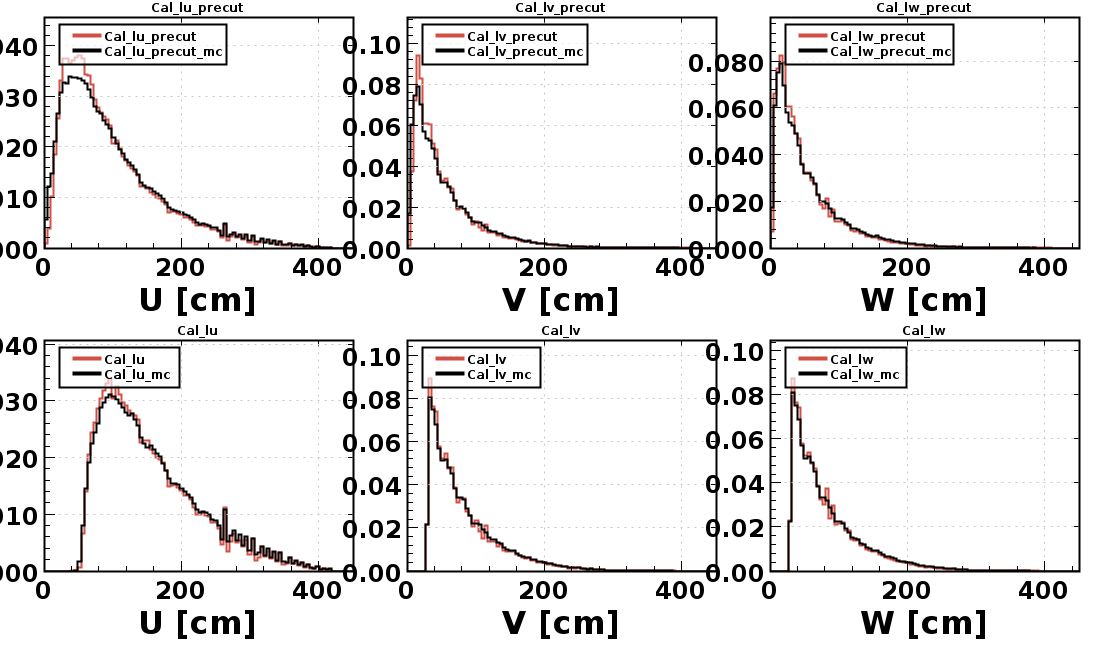
\includegraphics[width=0.9\linewidth]{figures/rga/1d_ecal.png}
	\caption{1D distributions of the U, V, and W sectors of the PCAL. The uncut histograms are on the top and the bottom histograms contain the cuts: $U<30$ cm, $30<V<390$ cm, and $30<W<390$ cm. All plots are normalized to account for any mismatch in total statistics. Red lines are from RGA data and black lines are for the Monte-Carlo (MC) data.}
	\label{fig:rga_1decal}
\end{figure}

\begin{figure}[h!]
	\centering
	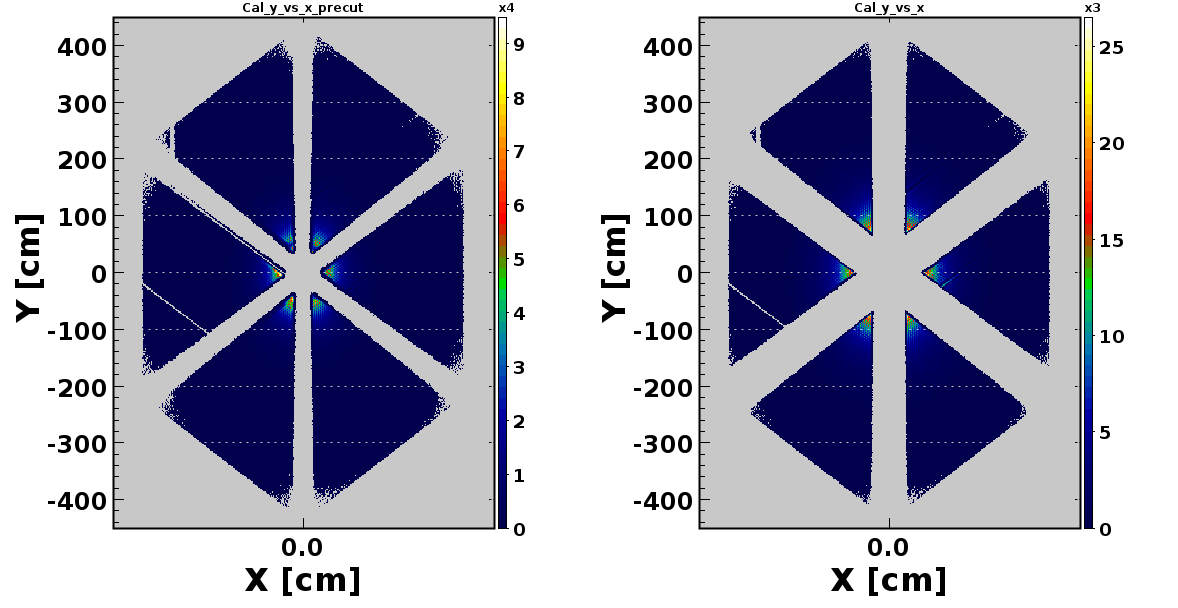
\includegraphics[width=0.9\linewidth]{figures/rga/2d_ecal.png}
	\caption{2D histograms of the uncut PCAL hits on the left and the 2D histogram containing the fiducial cuts.}
	\label{fig:rga_2decal}
\end{figure}

The EC is the detector that we use for determining the electron four-momentum and all kinematics that are calculated from that momentum. When electrons enter the EC they shower and stop. That EM shower is broad, so we have to remove events close to the edges as showers leak out and the sampling fraction becomes unreliable for $e^-$ PID.

Remember that the EC sector is defined by U, V, and W edges of its triangular shape. We can cut on those edges for the PCAL only and the effects will propagate through to the EC$_{\mathrm{inner}}$ (ECin) and EC$_{\mathrm{outer}}$ (ECout). The established cuts for the PCAL are $U<30$ cm, $30<V<390$ cm, and $30<W<390$ cm. Fig. \ref{fig:rga_1decal} shows the one-dimensional distributions of the U, V, and W sectors of the PCAL. The uncut histograms are on the top and the bottom histograms contain the cuts that were described. Fig. \ref{fig:rga_2decal} contains the two-dimensional histograms of the uncut PCAL hits on the left and the 2D histogram containing the fiducial cuts.

\section{Kinematic Cuts}
Our goal is to extract the inclusive DIS cross section for the process $ep \longrightarrow e'X$, which means that certain constraints must be put on some of the kinematic variables. To isolate DIS events, $W>2$ GeV and $Q^2>1$ GeV$^2$. Other \textit{kinematic cuts} must be applied. In order to isolate events that originate at the target, we require $-10 \mathrm{cm} < v_z < 10 \mathrm{cm}$, where $v_z$ is the z-vertex position of the track. Fig. \ref{fig:rga_vz} shows $v_z$ before (left) and after (right) cuts. Because there is no discernible difference between left and right (uncut and cut), it is clear that cuts were made during reconstruction.

\begin{figure}[h!]
	\centering
	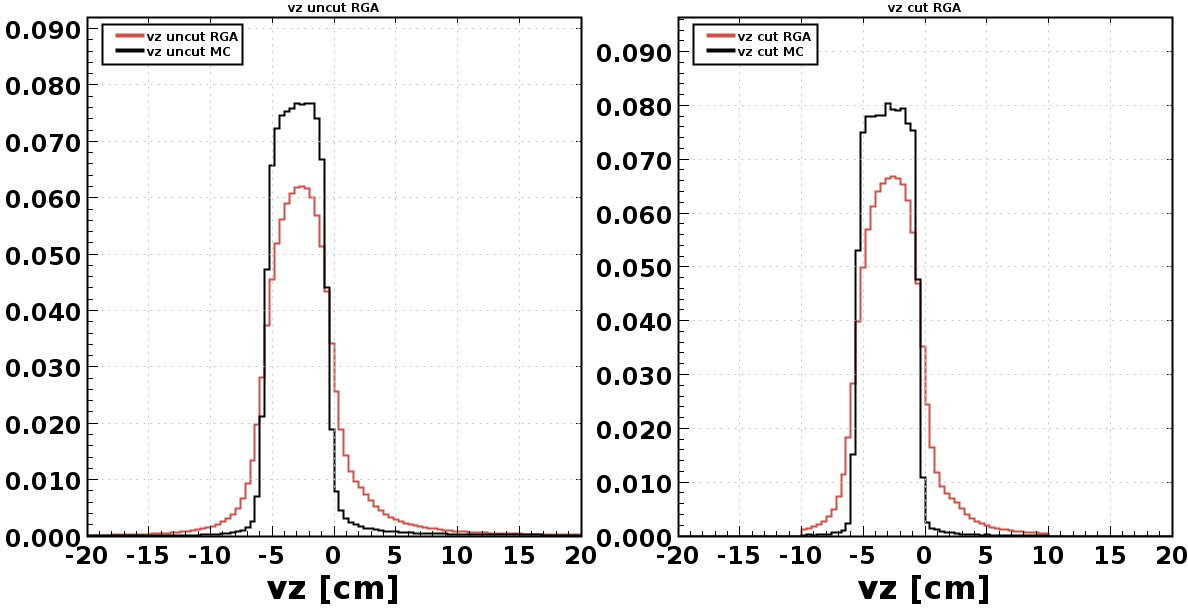
\includegraphics[width=0.9\linewidth]{figures/rga/vz.png}
	\caption{$v_z$ before and after all described cuts. Red lines are from RGA data and black lines are for the Monte-Carlo (MC) data.}
	\label{fig:rga_vz}
\end{figure}

\begin{figure}[h!]
	\centering
	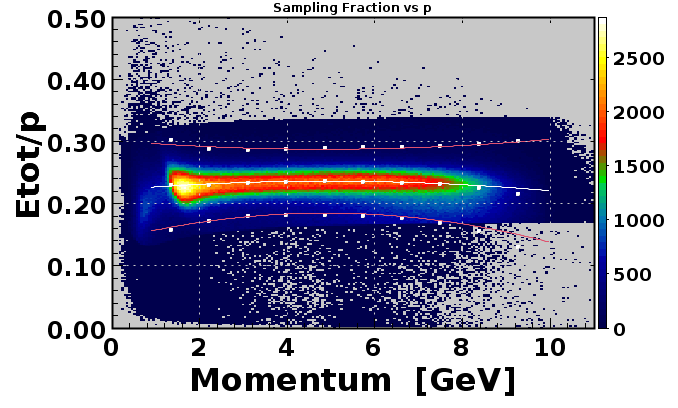
\includegraphics[width=0.9\linewidth]{figures/rga/fit_etot_p.png}
	\caption{Slicing and fitting of the sampling fraction to create a $5\sigma$ cut.}
	\label{fig:rga_etot_p}
\end{figure}

The last significant kinematic cut occurs on the sampling faction. The sampling fraction is defined as $E_{tot}/p$, where $E_{tot}$ is the total energy deposited by the particle in all three layers of the EC and $p$ is the particle's momentum. When the sampling fraction is plotted vs $p$, electrons will appear as a band around 0.25 and with a momentum of above 1 GeV to eliminate any minimum ionizing particles like pions. To do this, we take slices of the plot, find the mean and sigma of $E_{tot}/p$ for that slice and cut out anything $\pm2.5\sigma$. We do this for values along $p$ and fit the points for means and $\pm2.5\sigma$ to polynomials that we can cut on to isolate electrons.

Because of the Forward Detector's coverage in $\theta$, we need to make sure that $5^{\circ} < \theta < 40^{\circ}$ so it falls within that coverage. Fig. \ref{fig:rga_kinematics_uncut} shows the uncut kinematic variables and Fig. \ref{fig:rga_kinematics_cut} was created with the kinematic cuts described. Fig. \ref{fig:rga_energies_uncut} and Fig. \ref{fig:rga_energies} shows uncut and cut (respectively) energy distributions for $E'$, EC, and the number of photoelectrons in the HTCC ($nphe$). The next group of plots Fig. \ref{fig:rga_2Dkin1_uncut}-\ref{fig:rga_sampFrac} shows two-dimensional histograms of various kinematic variables all uncut and after applying all cuts. In Fig. \ref{fig:rga_sampFrac} one can clearly see the successful application of the $5\sigma$ cut described in the previous paragraph.

The summary of applied cuts is as follows:
\begin{itemize}
	\item $W>2$ GeV
	\item $Q^2>1$ GeV$^2$
	\item $5^{\circ} < \theta < 40^{\circ}$
	\item PCAL fiducial cuts: $U<30$ cm, $30<V<390$ cm, and $30<W<390$ cm
	\item $-10<v_z<10$ cm
	\item $5\sigma$ cut on sampling fraction
	\item HTCC cut: $nphe > 5$
	\item EC energy cuts: $E_{\mathrm{PCAL}} > 0.06$ GeV, $E_{\mathrm{EC_{in}}} > 0.025$ GeV, $E_{\mathrm{EC_{out}}} > 0.05$ GeV
\end{itemize}

\begin{figure}[h!]
	\centering
	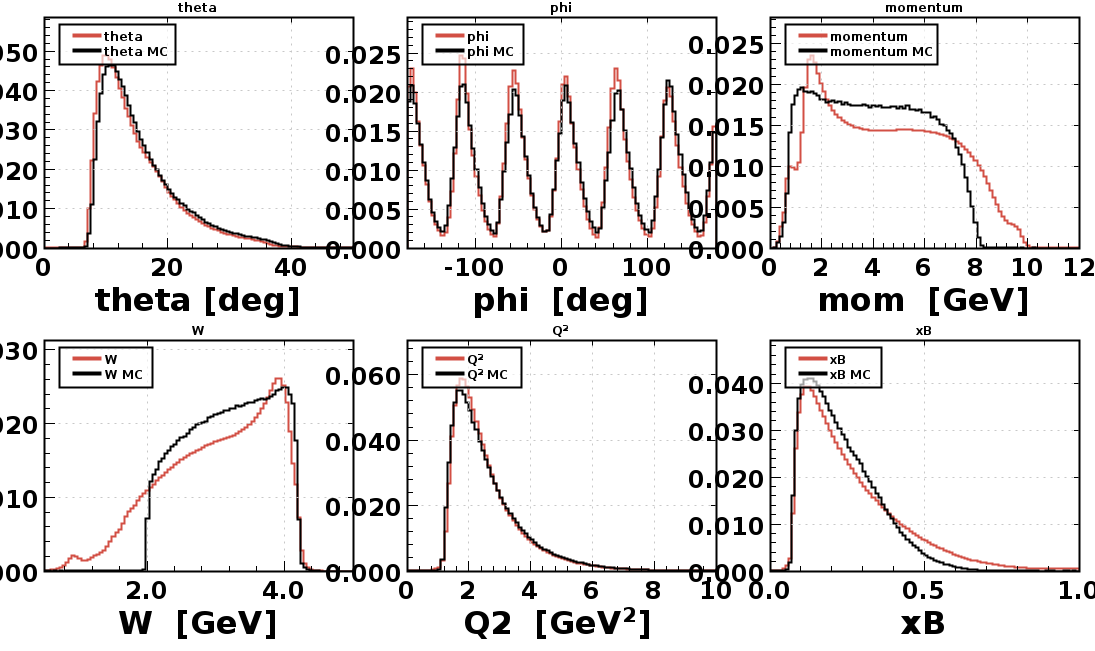
\includegraphics[width=0.9\linewidth]{figures/rga/uncut/kinematics.png}
	\caption{Kinematics variables before cuts. Red lines are from RGA data and black lines are for the Monte-Carlo (MC) data.}
	\label{fig:rga_kinematics_uncut}
\end{figure}

\begin{figure}[h!]
	\centering
	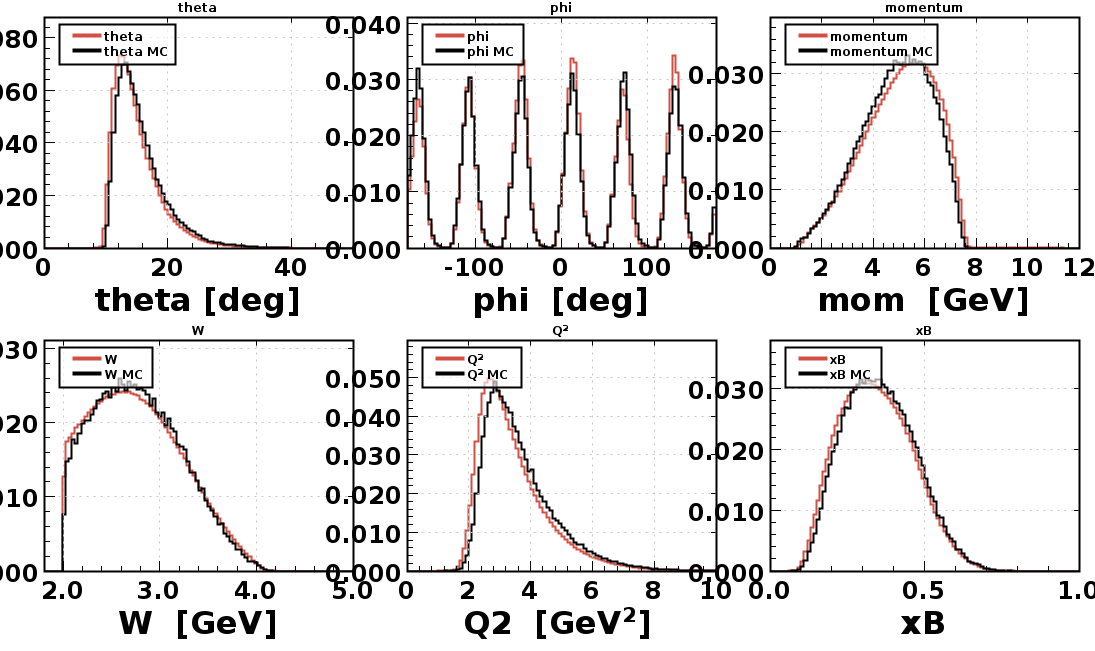
\includegraphics[width=0.9\linewidth]{figures/rga/kinematics.png}
	\caption{Kinematics variables after all described cuts. Red lines are from RGA data and black lines are for the Monte-Carlo (MC) data.}
	\label{fig:rga_kinematics_cut}
\end{figure}

\newpage
\begin{figure}[h!]
	\centering
	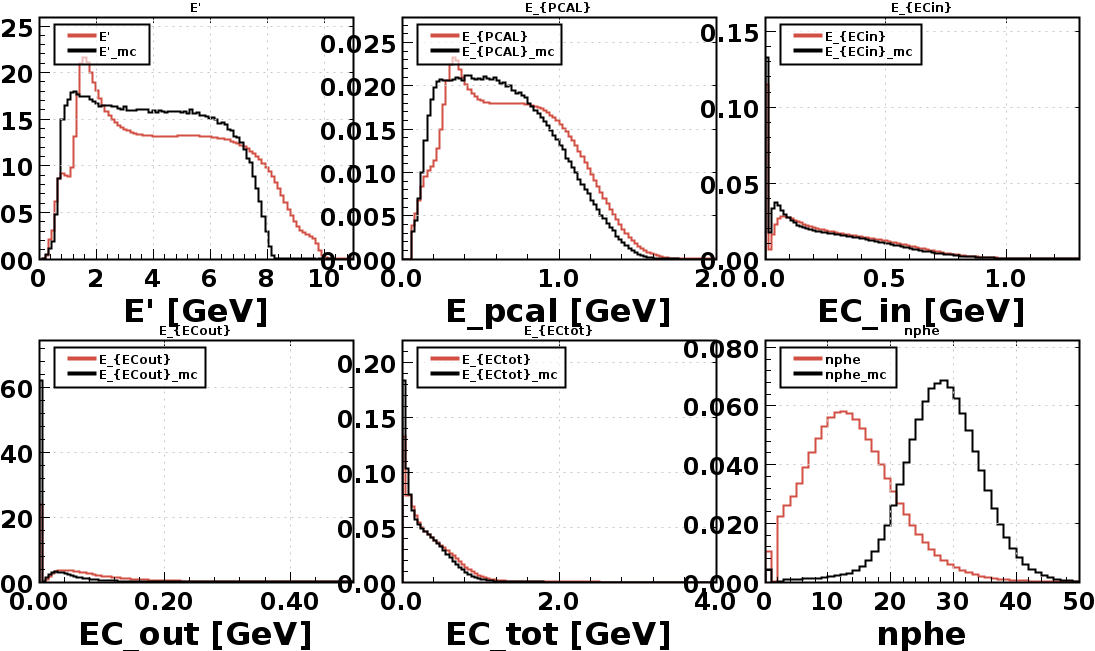
\includegraphics[width=0.9\linewidth]{figures/rga/uncut/energies.png}
	\caption{E' and EC energies before cuts. Red lines are from RGA data and black lines are for the Monte-Carlo (MC) data.}
	\label{fig:rga_energies_uncut}
\end{figure}

\begin{figure}[h!]
	\centering
	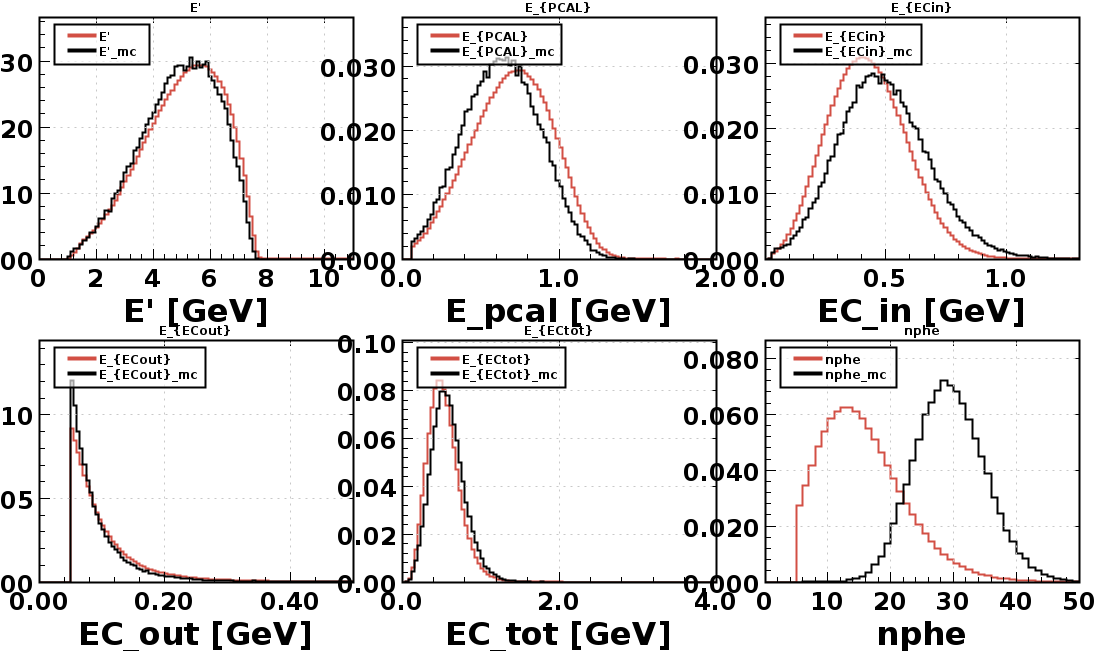
\includegraphics[width=0.9\linewidth]{figures/rga/energies.png}
	\caption{E' and EC energies after all described cuts. Red lines are from RGA data and black lines are for the Monte-Carlo (MC) data.}
	\label{fig:rga_energies}
\end{figure}

\newpage
\begin{figure}[h!]
	\centering
	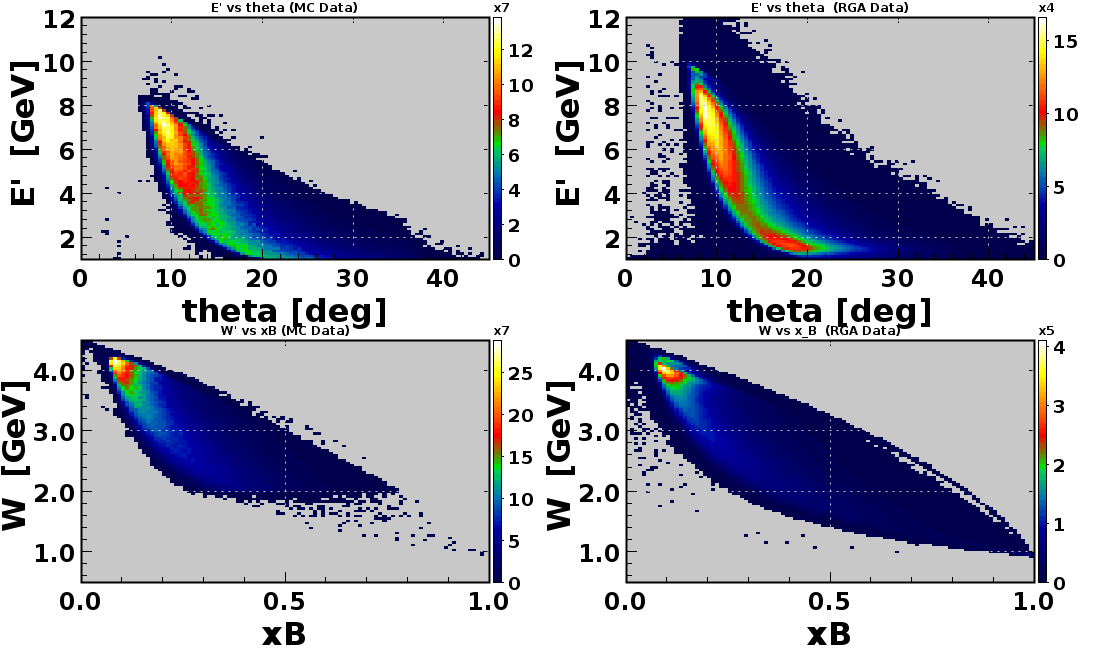
\includegraphics[width=0.9\linewidth]{figures/rga/uncut/2Dkin1.png}
	\caption{$E'$ vs. $\theta$ and $W$ vs. $x_B$ before cuts.}
	\label{fig:rga_2Dkin1_uncut}
\end{figure}

\begin{figure}[h!]
	\centering
	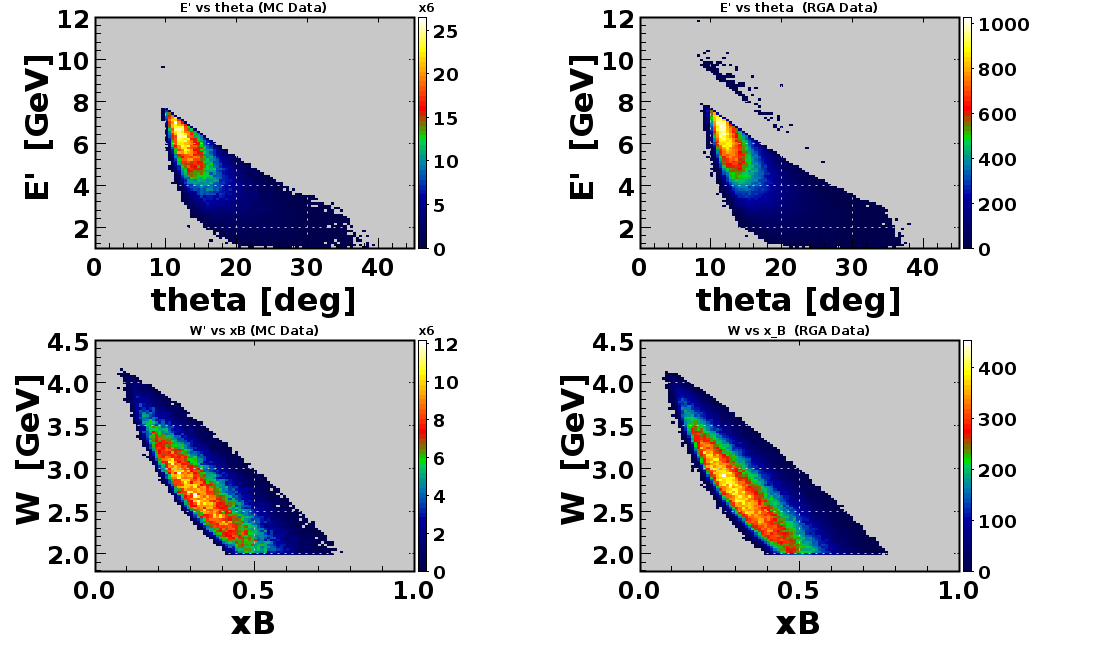
\includegraphics[width=0.9\linewidth]{figures/rga/2Dkin1.png}
	\caption{$E'$ vs. $\theta$ and $W$ vs. $x_B$ after all described cuts.}
	\label{fig:rga_2Dkin1}
\end{figure}

\newpage
\begin{figure}[h!]
	\centering
	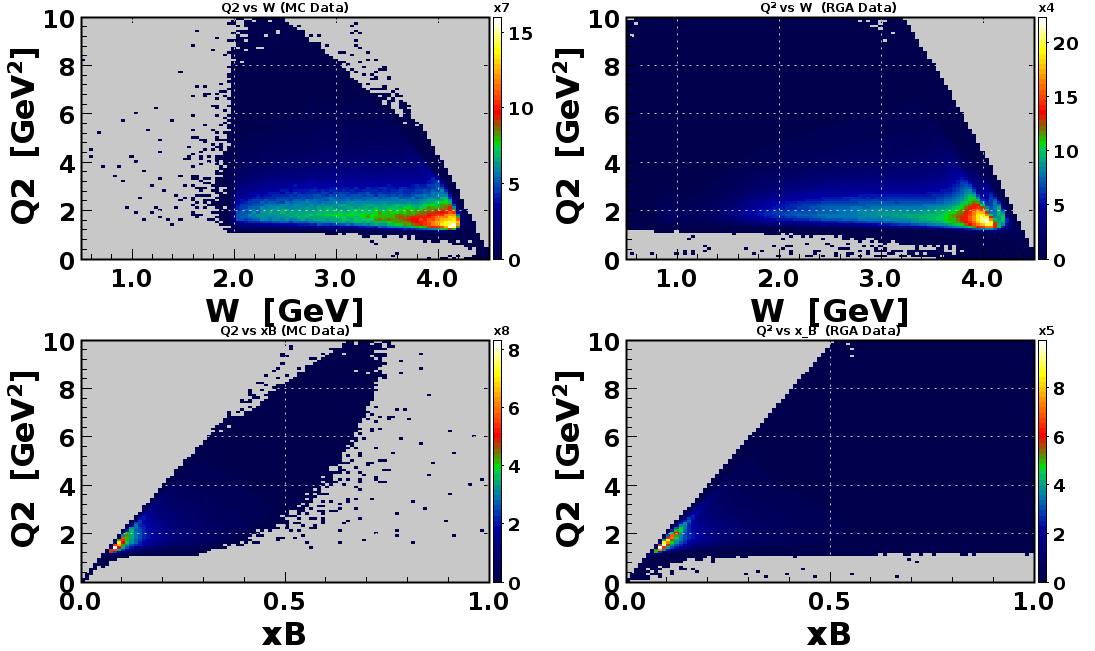
\includegraphics[width=0.9\linewidth]{figures/rga/uncut/2Dkin2.png}
	\caption{$Q^2$ vs. $W$ and $Q^2$ vs $x_B$ before cuts.}
	\label{fig:rga_2Dkin2_uncut}
\end{figure}

\begin{figure}[h!]
	\centering
	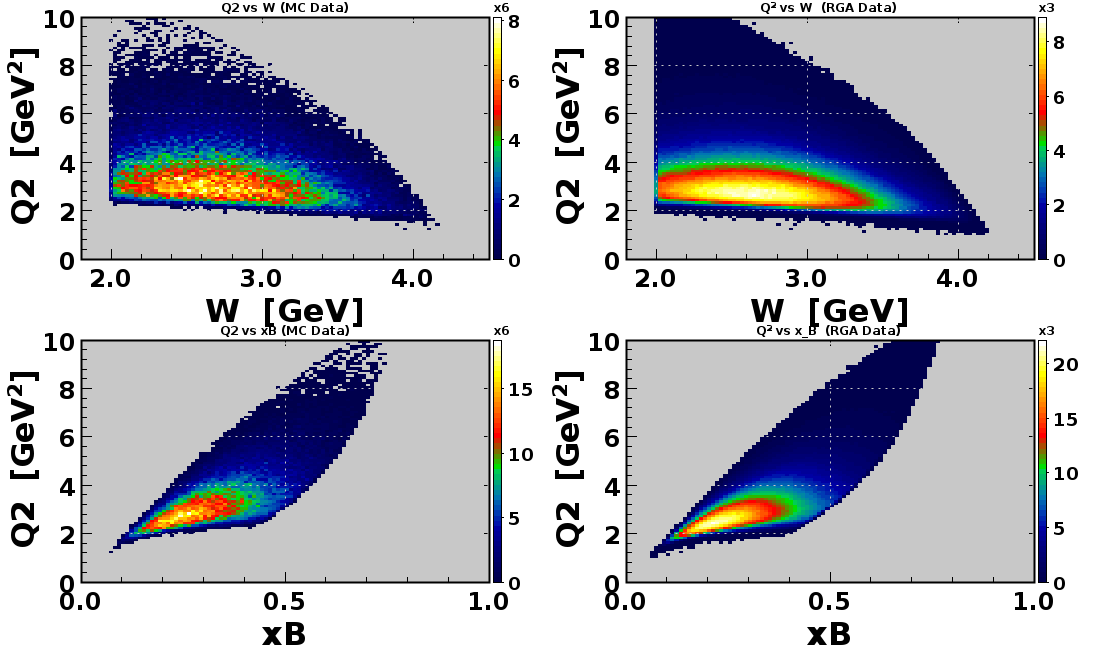
\includegraphics[width=0.9\linewidth]{figures/rga/2Dkin2.png}
	\caption{$Q^2$ vs. $W$ and $Q^2$ vs $x_B$ after all described cuts.}
	\label{fig:rga_2Dkin2}
\end{figure}

\newpage
\begin{figure}[h!]
	\centering
	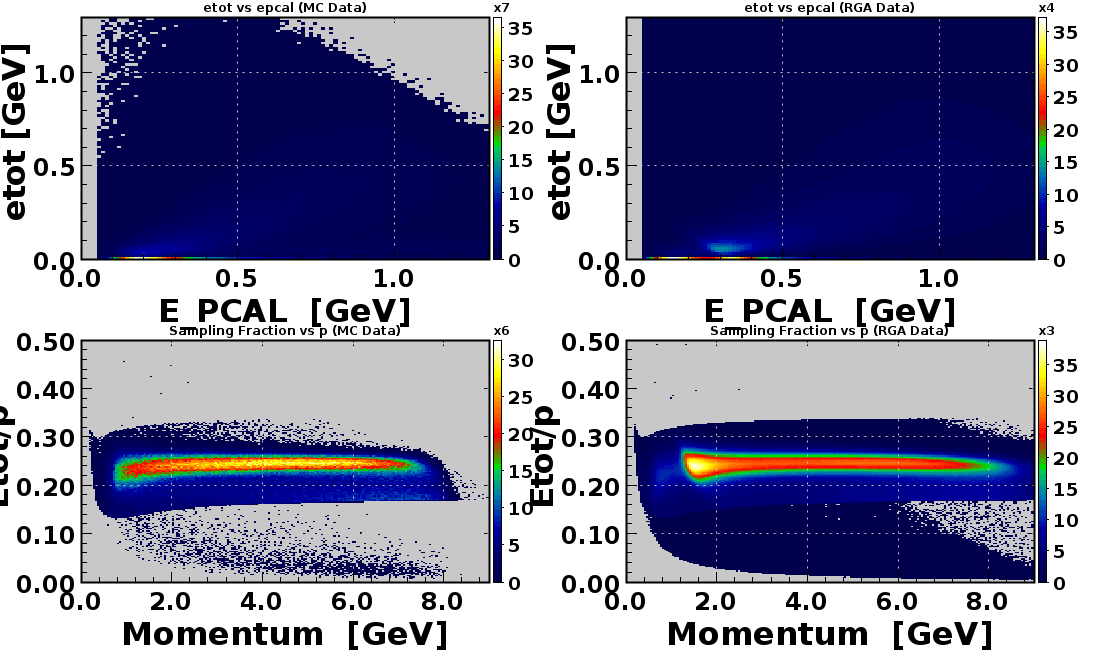
\includegraphics[width=0.9\linewidth]{figures/rga/uncut/sampFrac.png}
	\caption{$E_{EC_{tot}}$ vs $E_{PCAL}$ and Sampling fraction before cuts.}
	\label{fig:rga_sampFrac_uncut}
\end{figure}

\begin{figure}[h!]
	\centering
	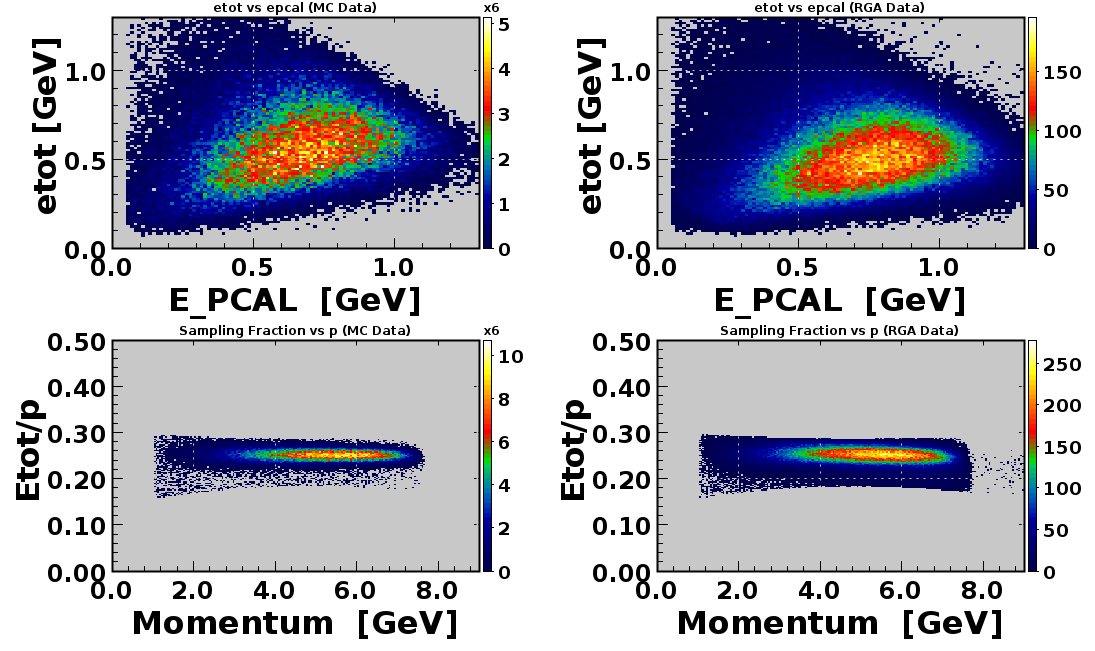
\includegraphics[width=0.9\linewidth]{figures/rga/sampFrac.png}
	\caption{$E_{EC_{tot}}$ vs $E_{PCAL}$ and Sampling fraction after all described cuts.}
	\label{fig:rga_sampFrac}
\end{figure}

\cleardoublepage
\section{Binning and Acceptance}
The data, after kinematic and fiducial cuts, needs to be separated into kinematic bins in order to first obtain the acceptance of the bin and then to extract the cross section for each bin. The acceptance for the bin is defined as
\begin{equation}
A(x,y) = \frac{N_{\mathrm{rec}}(x,y)}{N_{\mathrm{gen}}(x,y)},
\end{equation}
where $A(x,y)$ is the acceptance of the bin, $N_{\mathrm{gen}}(x,y)$ is the number of generated events in that bin, and $N_{\mathrm{rec}}(x,y)$ is the number of reconstructed events in that bin. The binning occurs in $x$ ($i.e.$ the Bjorken-$x$ scaling variable) and $y$, which is defined as $y = \nu/E$. This particular binning was done because of the cross section calculation that was done using model by Christy-Bosted, namely:
\begin{equation}
\label{eq:dis_xsec}
\frac{d^2\sigma}{dxdy} = \frac{4\pi\alpha_{\mathrm{em}}S}{Q^4} \left[ xy^2 F_1(x,Q^2) + \left( 1-y-xy\frac{M^2}{S} \right) F_2(x,Q^2) \right],
\end{equation}
where $S = 2ME$.

\begin{figure}[h!]
	\centering
	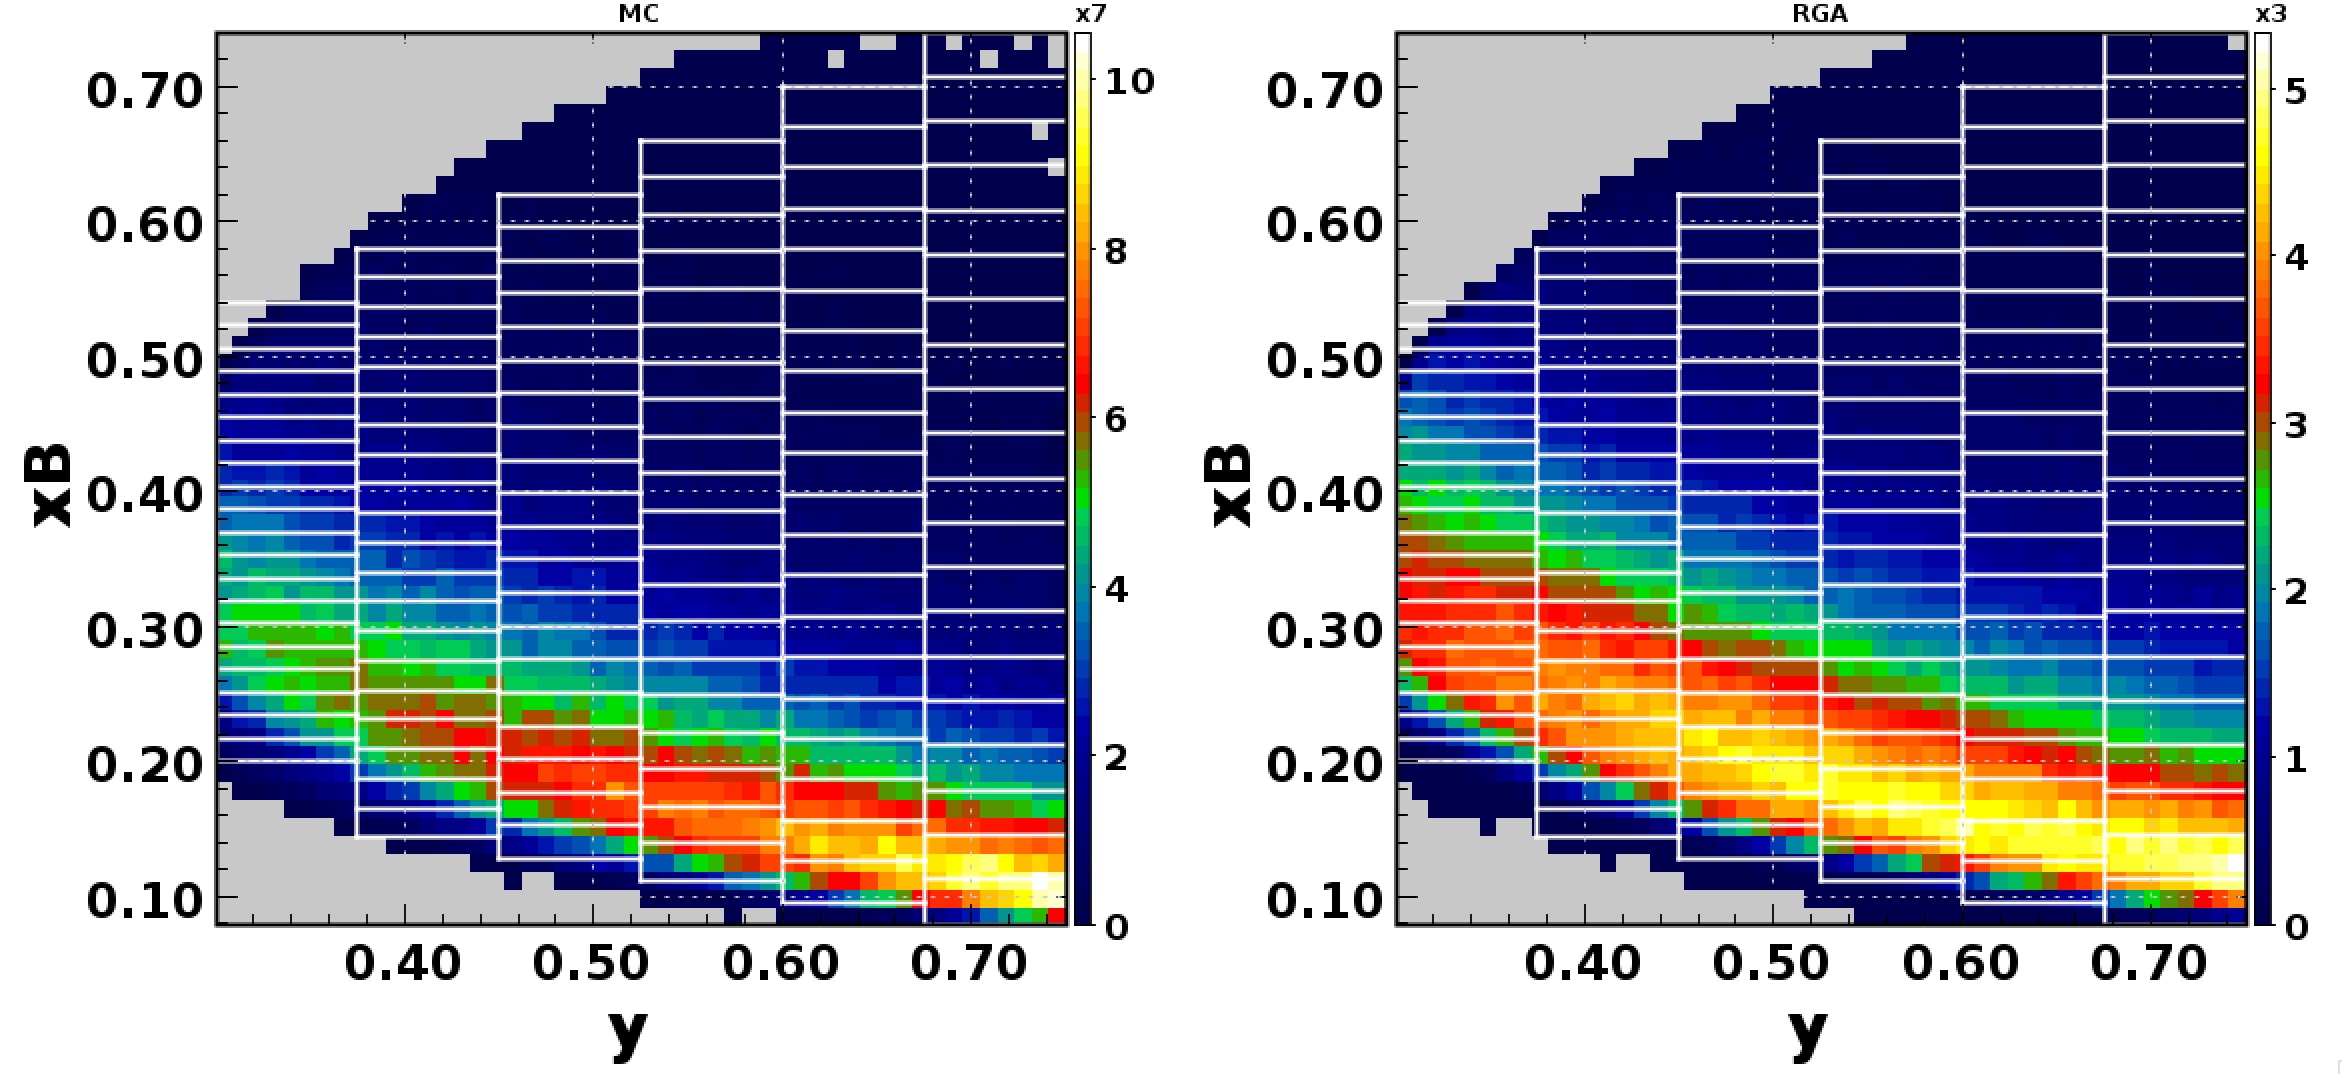
\includegraphics[width=0.9\linewidth]{figures/rga/xB_vs_y_bins.png}
	\caption{Binning in the $x,y$ space.}
	\label{fig:xb_vs_y_bins}
\end{figure}

The binning in $x$ and $y$ was done in an attempt to gather equal statistics in each bin. Equal bins were chosen in $y$ because, in the range $0.3 < y < 0.74$, the distribution was relatively flat. In $x$, however, the shape of the distribution required tuned binning throughout. Table \ref{table:xB_bins} outlines the bin size and range for $x$. Fig. \ref{fig:xb_vs_y_bins} shows the binning in the $x,y$ space. 

\begin{table}[h!]
	\centering
	\begin{tabular}{ |c|c|c|c|c| } 
		\hline
		Bin & $y$ Range & $x_{\mathrm{min}}$ & $x_{\mathrm{max}}$ & $\Delta x$ \\
		\hline
		1 & 0.3, 0.375 & 0.2 & 0.54 & 0.17 \\
		2 & 0.375, 0.45 & 0.144 & 0.58 & 0.0218 \\
		3 & 0.45, 0.525 & 0.128 & 0.62 & 0.0246 \\
		4 & 0.525, 0.6 & 0.112 & 0.66 & 0.0274 \\
		5 & 0.6, 0.675 & 0.096 & 0.7 & 0.0302 \\
		6 & 0.675, 0.75 & 0.08 & 0.74 & 0.033 \\
		\hline
	\end{tabular}
	\caption{Summary of binning in $x$ and $y$.}
	\label{table:xB_bins}
\end{table}

Figs. \ref{fig:rga_acc0}-\ref{fig:rga_acc2} show the acceptance for each bin. For each bin in $y$, the value of which is located at the top of each plot, the acceptance is then plotted for each bin in $x$. Ideally the acceptance for all bins would be unity, so it is clear that the acceptance in areas of high and low $y$ is lacking. In Fig. \ref{fig:rga_acc0} we see that the acceptance is low at $x \rightarrow 0$ and in Fig. \ref{fig:rga_acc2} acceptance drops as $x \rightarrow 1$. 

\begin{figure}[h!]
	\centering
	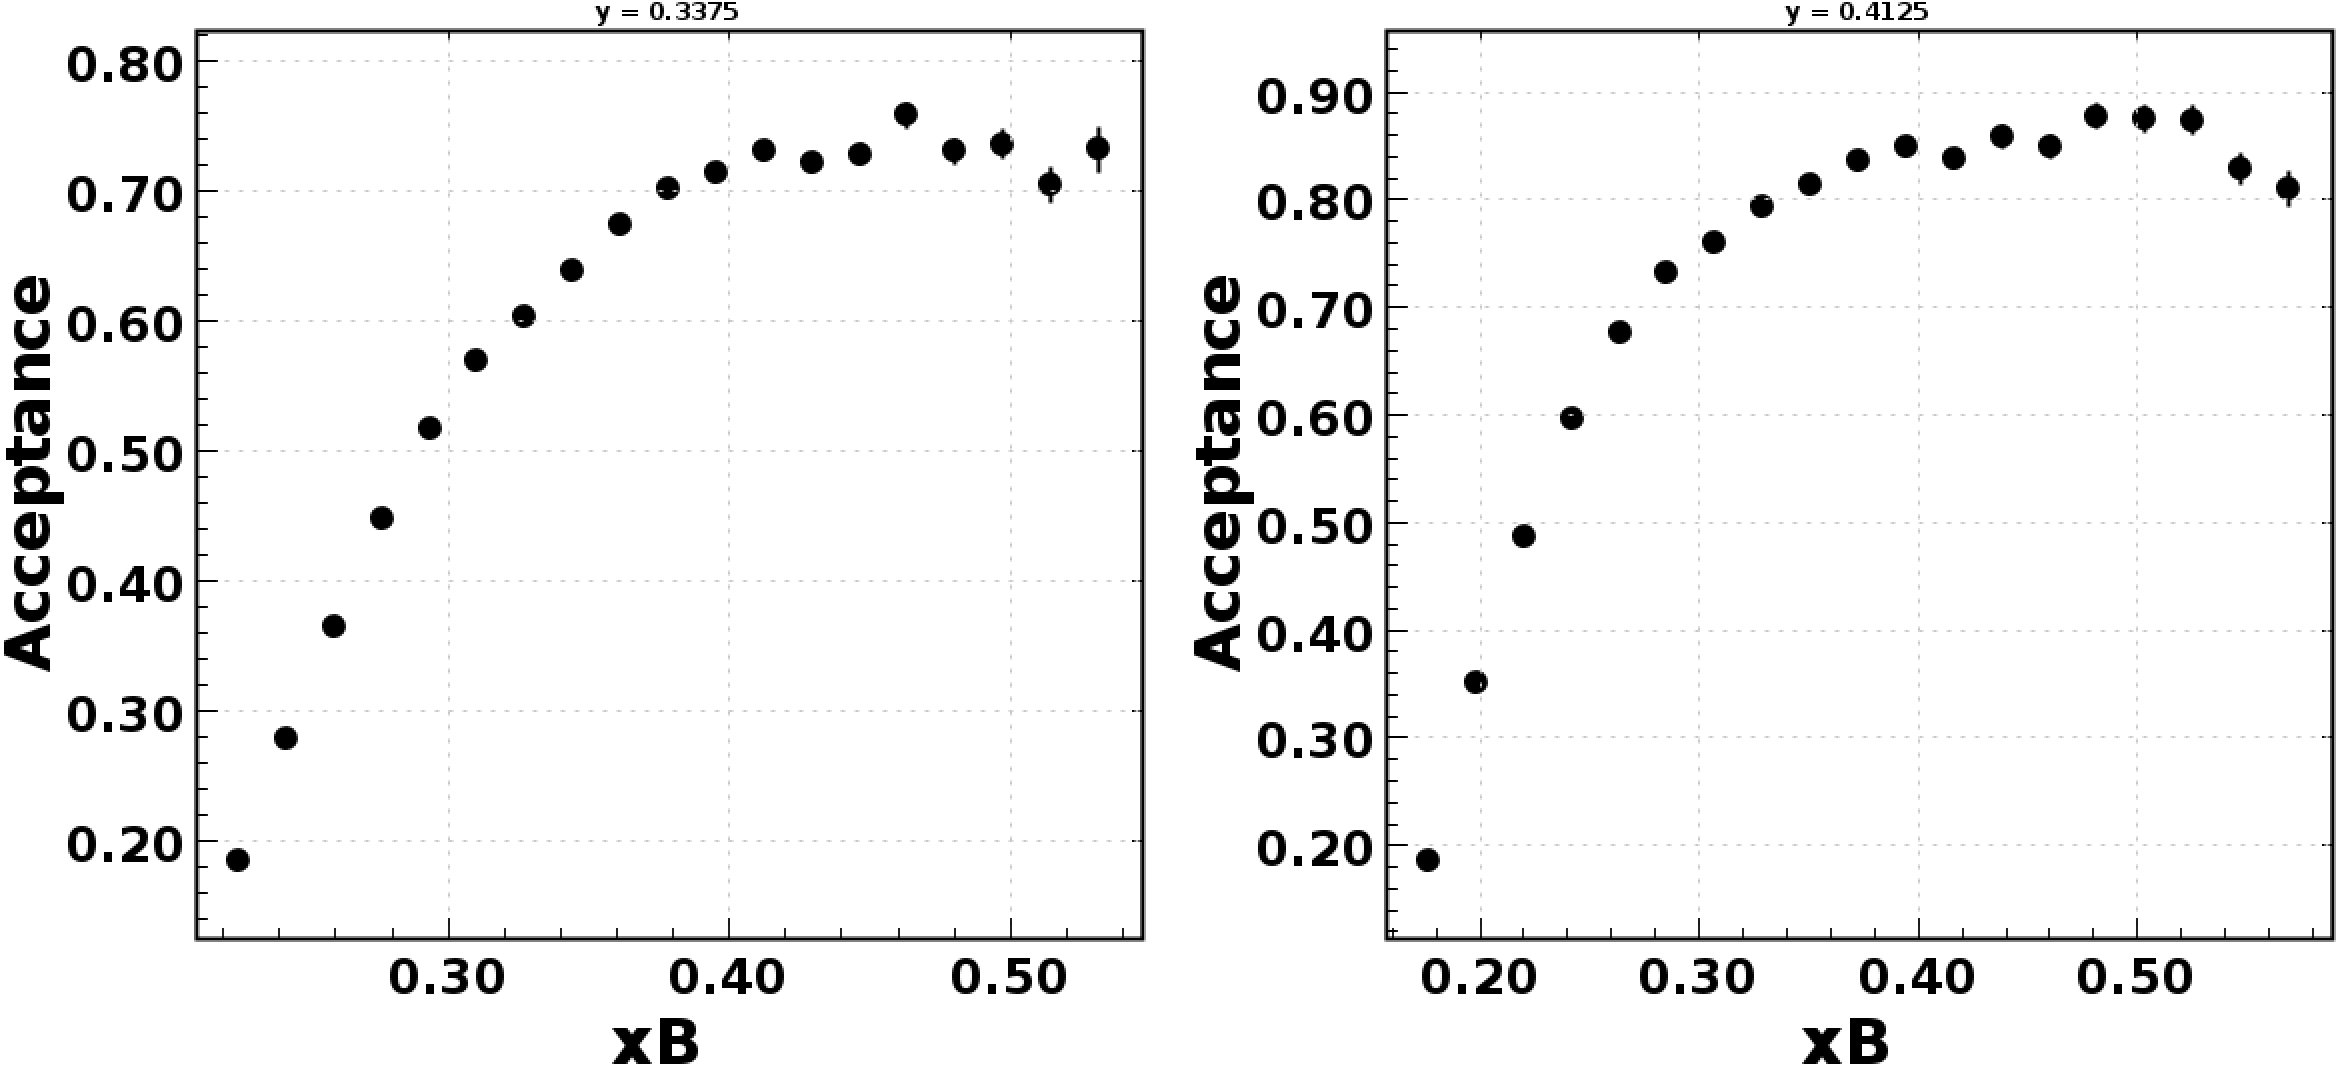
\includegraphics[width=0.9\linewidth]{figures/rga/acceptance0.png}
	\caption{}
	\label{fig:rga_acc0}
\end{figure}
\begin{figure}[h!]
	\centering
	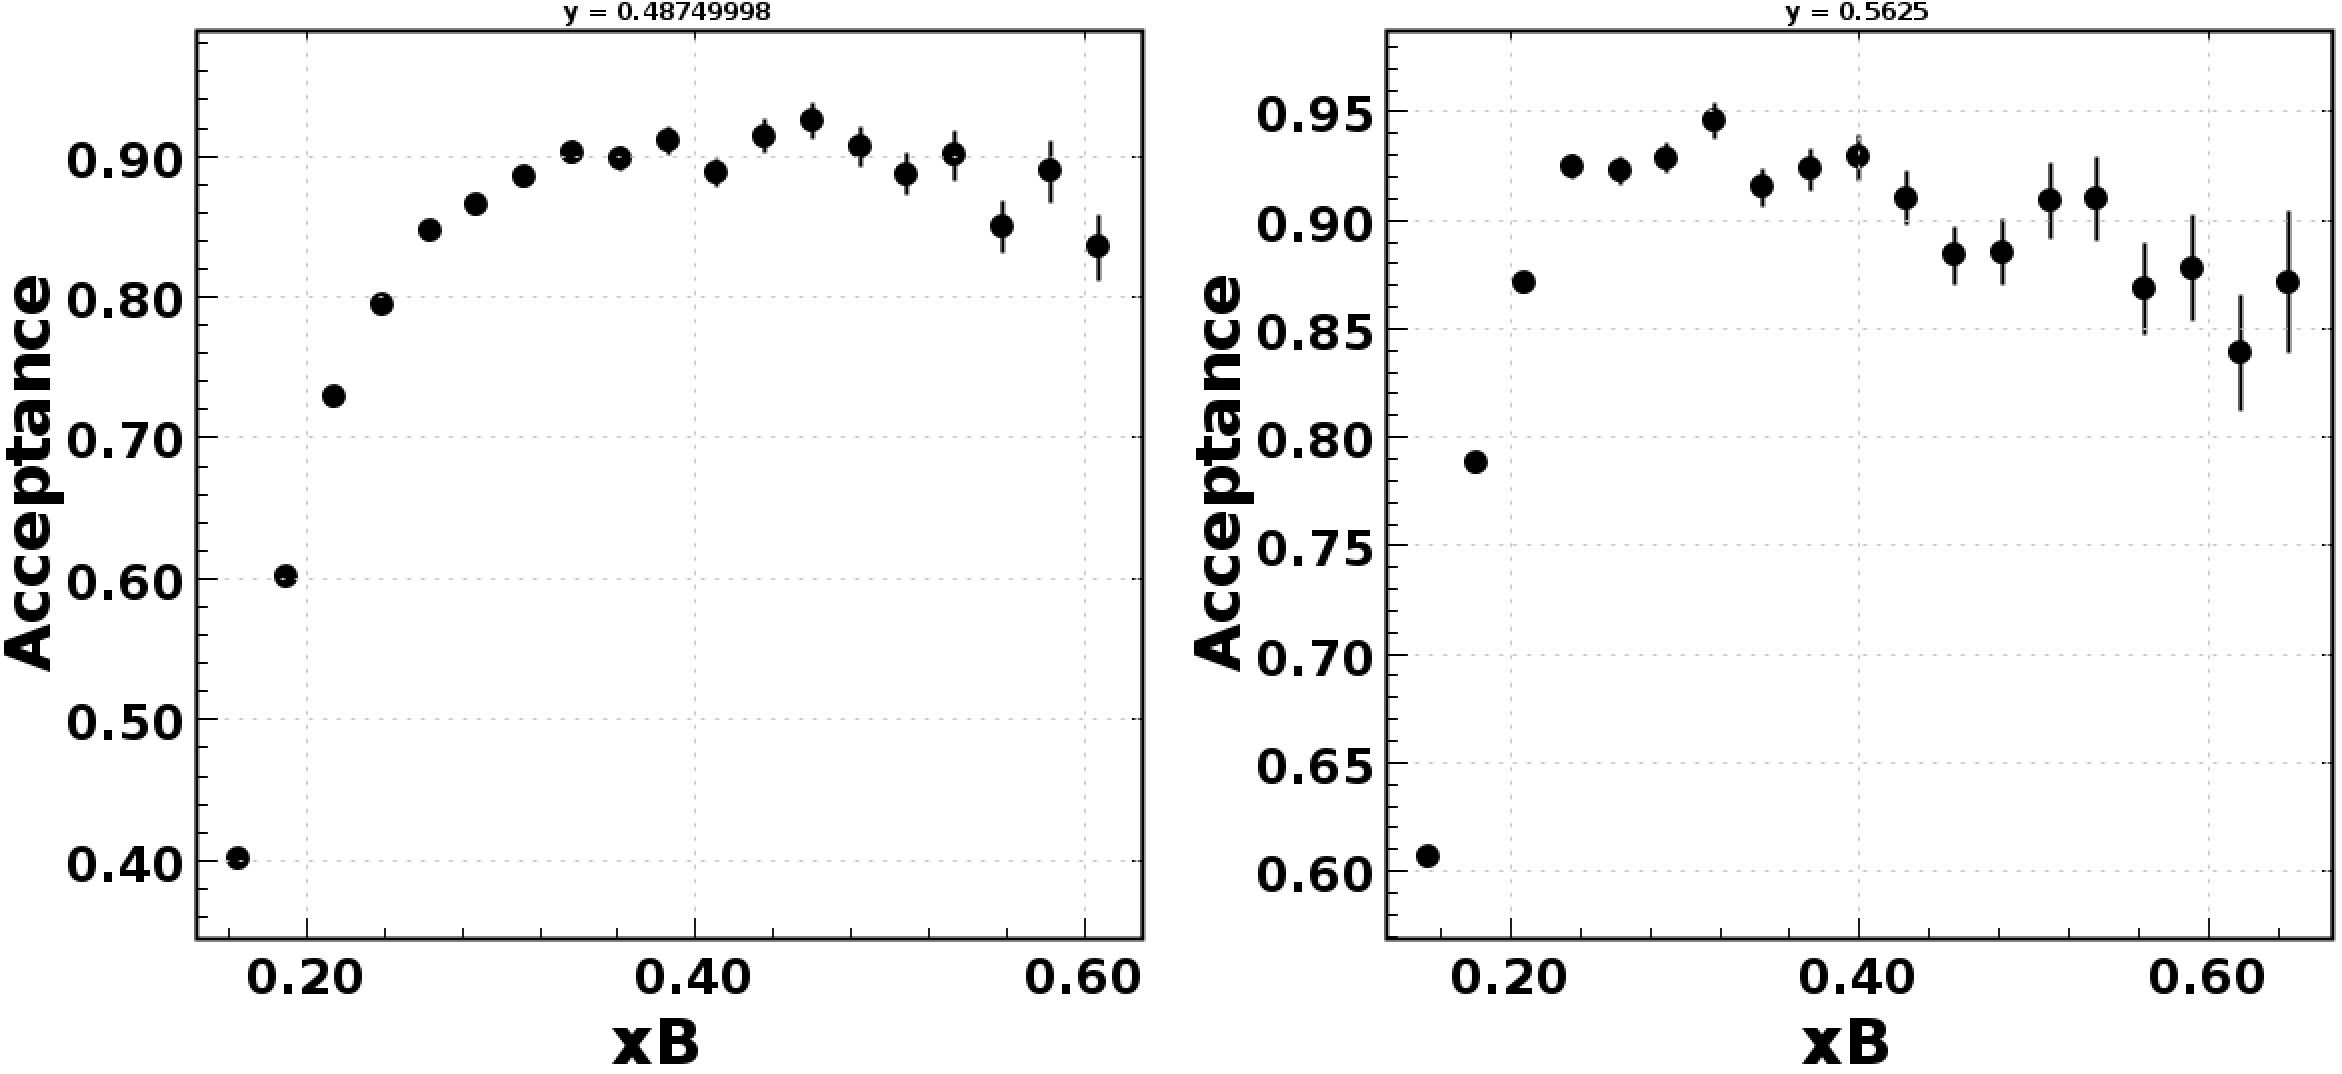
\includegraphics[width=0.9\linewidth]{figures/rga/acceptance1.png}
	\caption{}
	\label{fig:rga_acc1}
\end{figure}
\begin{figure}[h!]
	\centering
	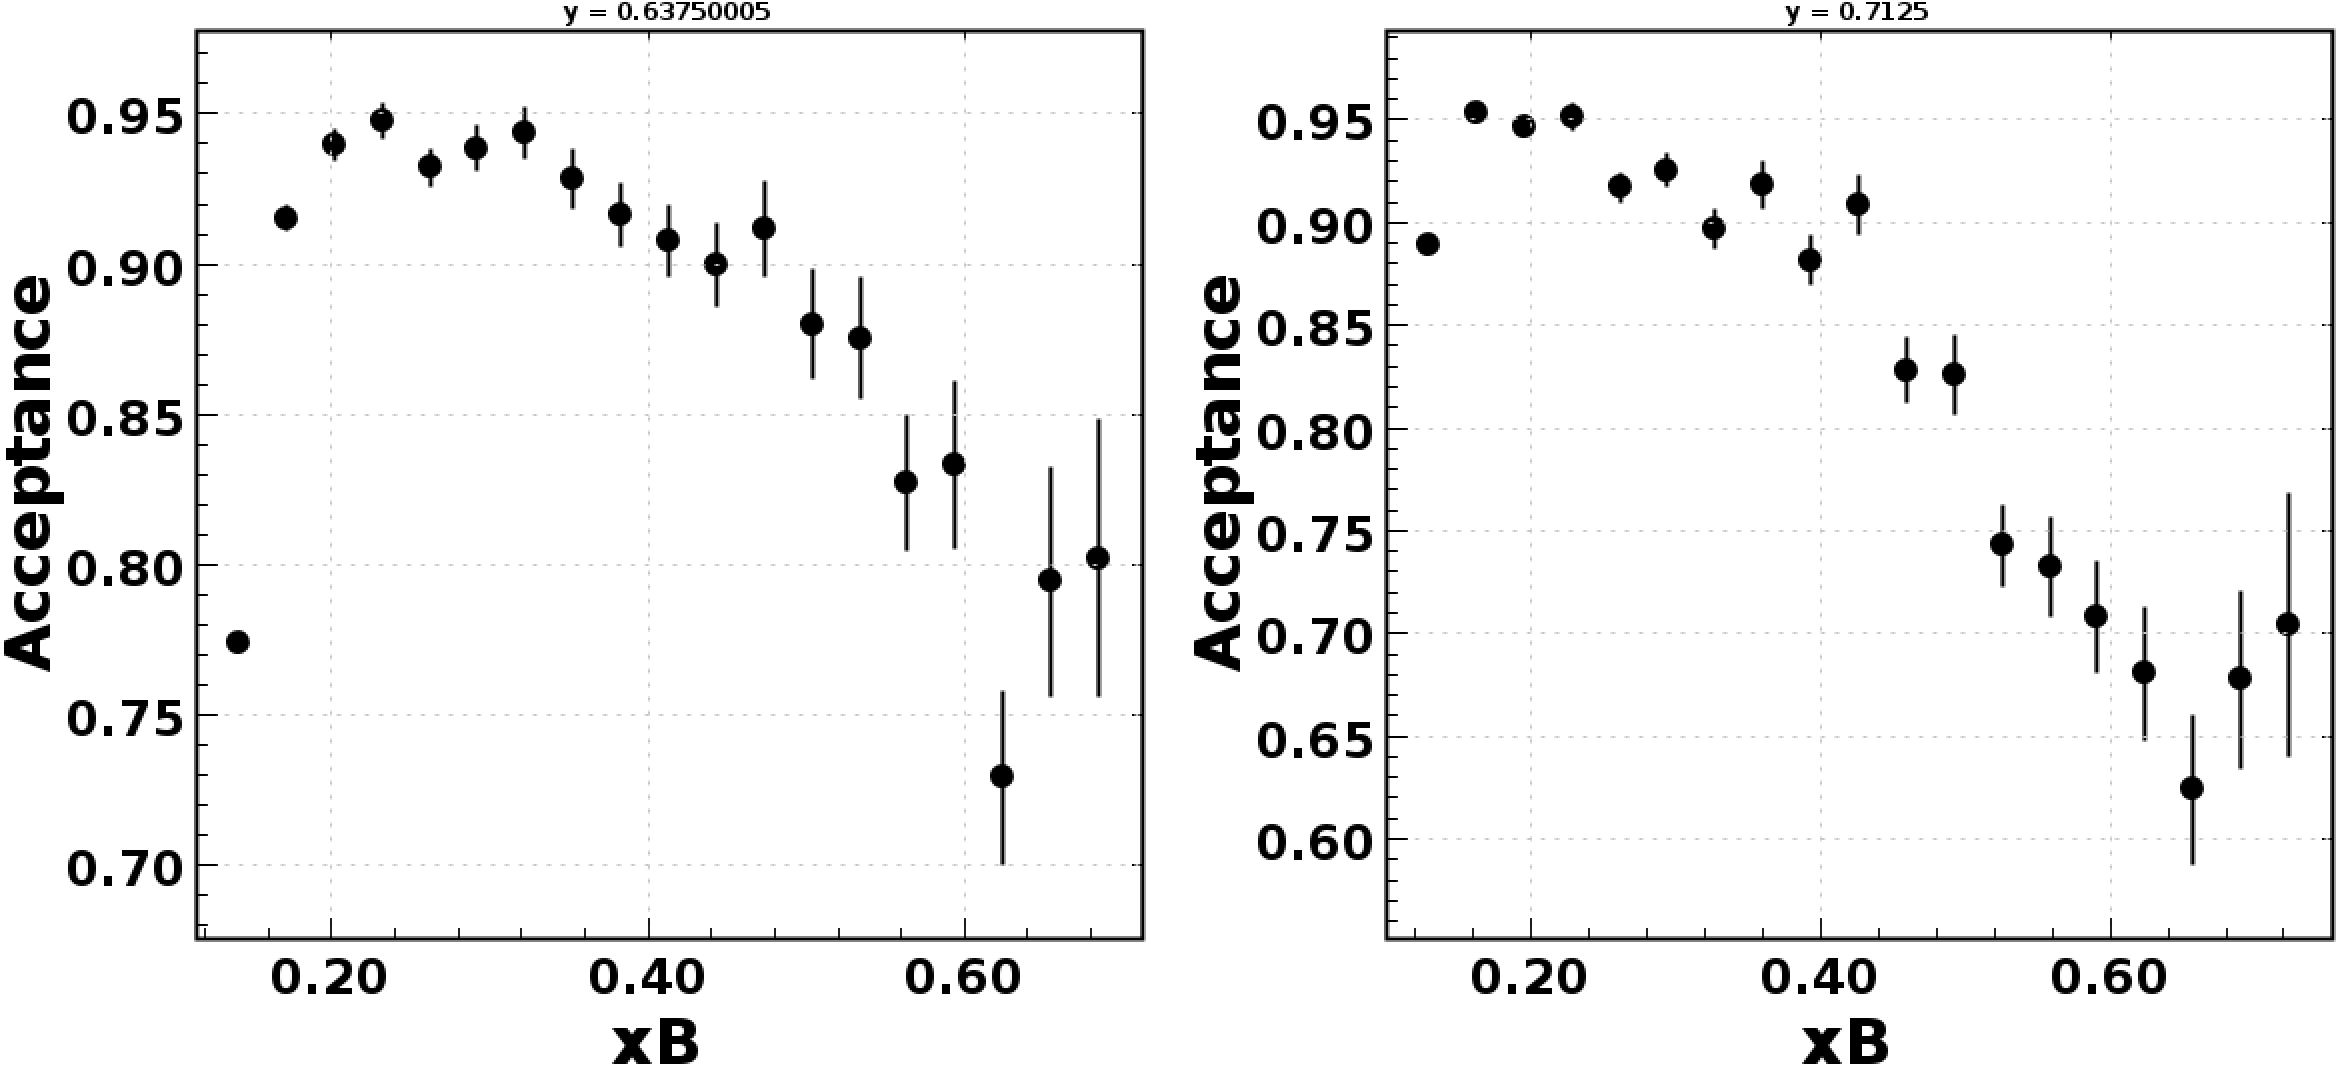
\includegraphics[width=0.9\linewidth]{figures/rga/acceptance2.png}
	\caption{}
	\label{fig:rga_acc2}
\end{figure}

\section{Faraday Cup and Integrated Luminosity}
As will become more evident in the next section, cross section calculations depend on the number of beam electrons accumulated during a particular run. Since that cross section is essentially the probability that a reaction occurs for a given process, it also depends on the number of target nuclei. The \textit{luminosity} ($\mathscr{L}$) is a value incorporates both accumulated charge and number of target nuclei by expressing the number of beam particles per time multiplied by the number of target nuclei per unit area. By integrating that luminosity over time, we can recover the total number of beam electrons multiplied by the number of target nuclei per unit area
\begin{equation}
\mathscr{L_{\mathrm{int}}} = \int \mathscr{L} \; dt = \frac{N_{B} \times N_{\mathrm{target}}}{A},
\end{equation}
where $N_{B}$ is the total number of incident electrons, $N_{\mathrm{target}}$ is the number of target nuclei, and $A$ is the cross-sectional area of the target. This time-integrated luminosity ($\mathscr{L}_{\mathrm{int}}$) depends on calculating $N_{\mathrm{target}}/A$ and knowing the total number of electrons incident on the target.

\begin{figure}[h!]
	\centering
	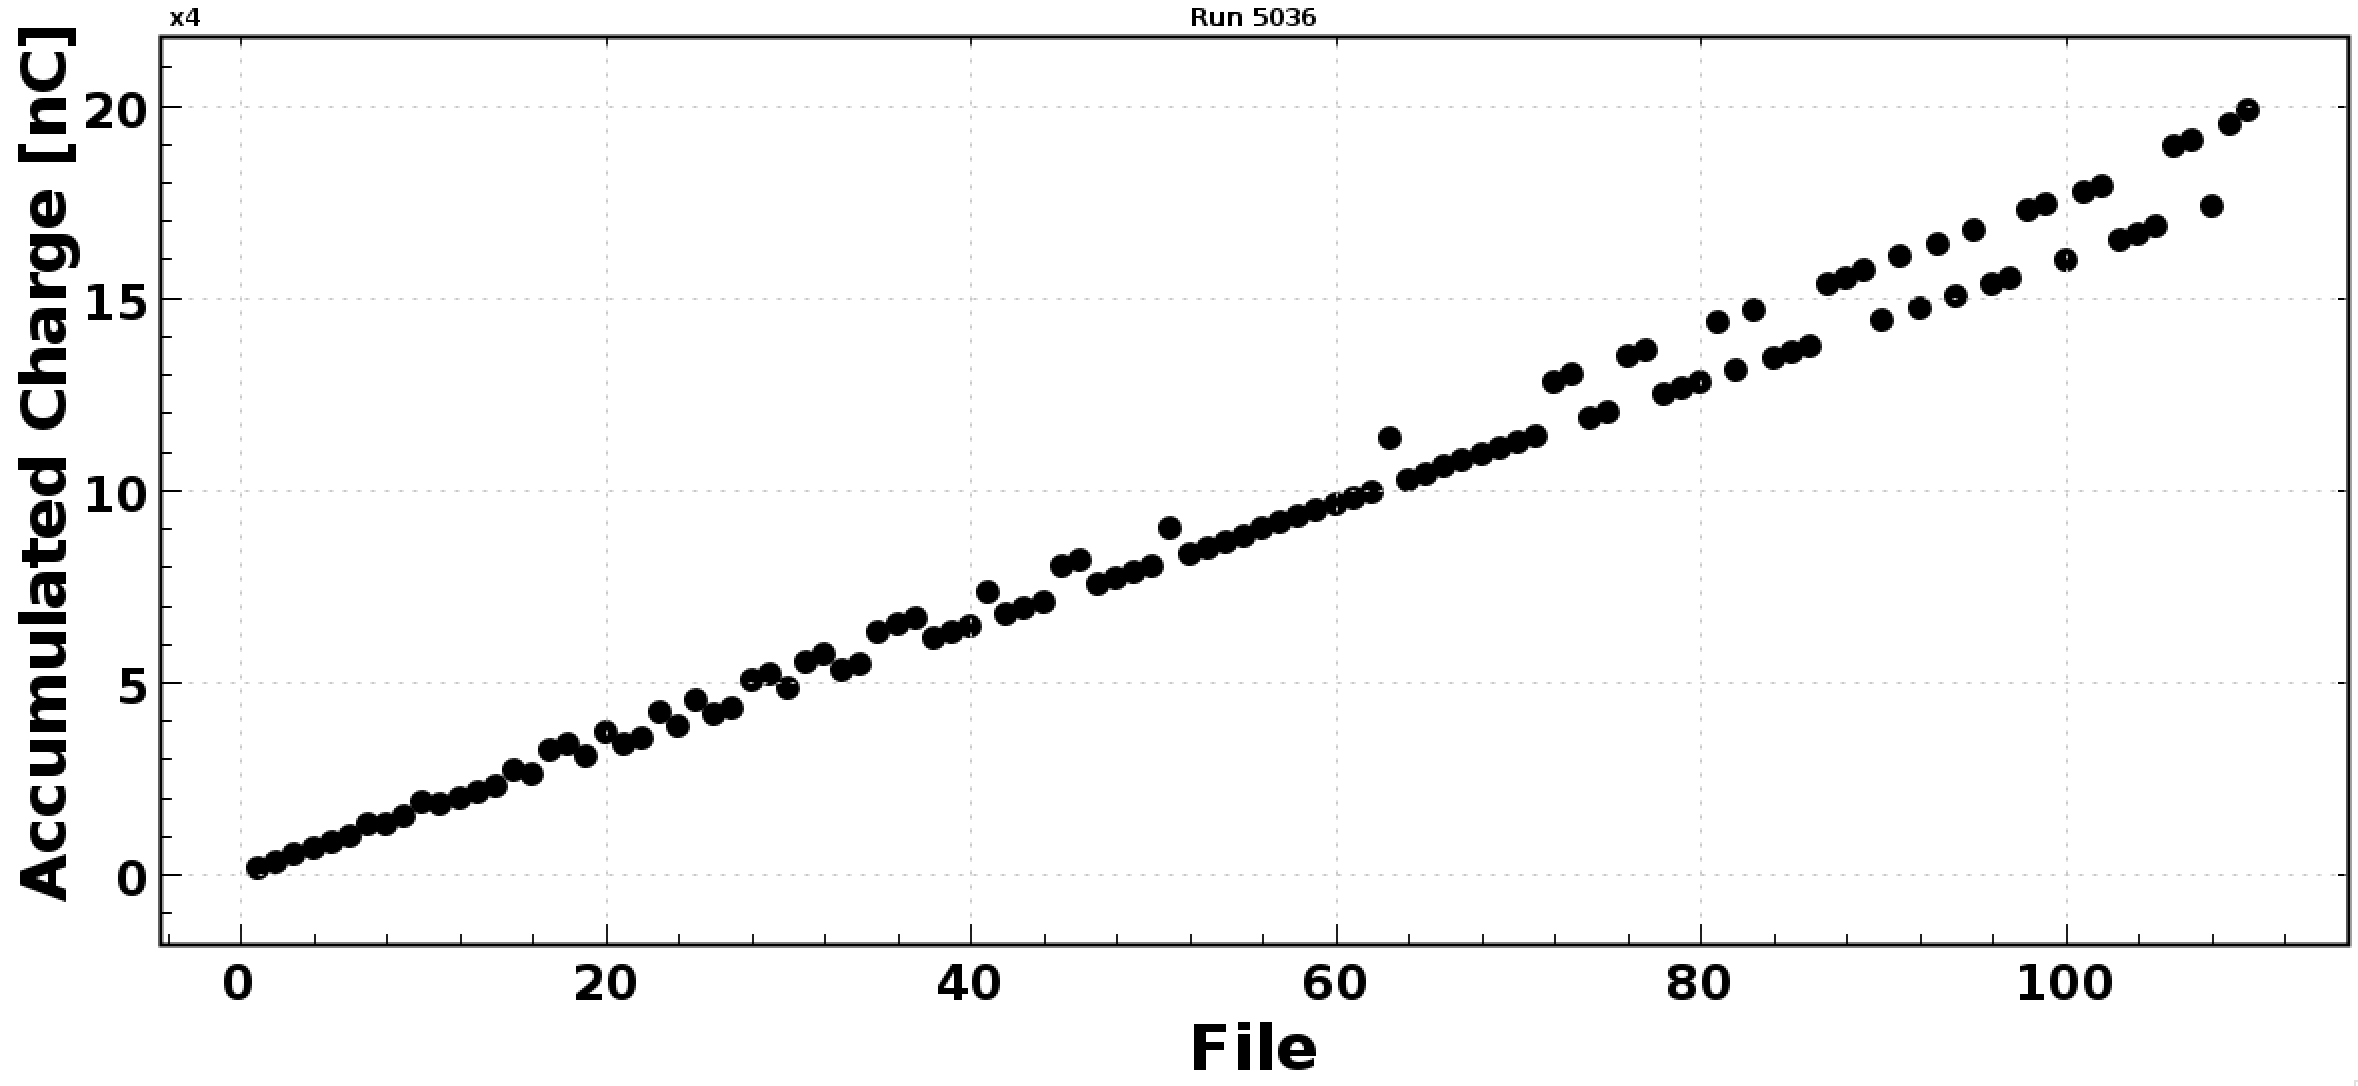
\includegraphics[width=0.9\linewidth]{figures/rga/charge.png}
	\caption{Accumulated charge vs. file for Run 5036.}
	\label{fig:rga_charge}
\end{figure}

Calculating the number of target nuclei per area can be done utilizing the ideal gas law
\begin{equation}
PV=nRT,
\end{equation}
where $P$ is the target pressure, $V$ is the volume of the target, $n$ is the amount of target material that exists (in moles), $R$ is the gas constant equal to 8.314472 J/K$\cdot$mol, and $T$ is the target temperature. We can rearrange the equation to get
\begin{equation}
N_{\mathrm{target}} = 2nN_A = \frac{2PVN_A}{RT},
\end{equation}
where $N_A = 6.0221 \times 10^{23}$ mol$^{-1}$ is Avogadro's number and the ``2" comes from there being two hydrogen atoms in the liquid hydrogen target used for Run Group A (RGA). Finally, in order to find $N_{\mathrm{target}}$ in terms of the target density $\rho$, we use the relation 
\begin{equation}
n = \frac{m}{M_m} = \frac{PV}{RT} \Rightarrow \rho = \frac{M_m P}{RT}
\end{equation}
or
\begin{equation}
\frac{P}{T} = \frac{\rho R}{M_m},
\end{equation}
where $M_m$ is the molar mass. That results in
\begin{equation}
N_{\mathrm{target}} = \frac{2\rho V N_A}{M_m}.
\end{equation} 
This gives us a time-integrated luminosity
\begin{equation}
\mathscr{L}_{\mathrm{int}} = \frac{2N_B N_A \ell \rho}{M_m},
\end{equation}
where $\ell$ is the length of the target.

The last variable to find is the total number of electrons $N_B$. We do this by accessing the charge accumulation in the Faraday Cup. The Faraday Cup (FC) is device located at the end of the beam line that catches charged particles, giving access to the total charge during a given period. The FC data is given in nano Coloumbs (nC) integrated over the entire run, where in every nC of charge there are 6.24150636309$\times 10^{9}$ electrons. Fig. \ref{fig:rga_charge} shows that accumulated charge as the number of files for the run 5036. That allows us to get the total number of incident electrons for each run, which is $N_B$ in our integrated luminosity.

\section{Cross section}
The final step is to actually calculate the differential cross section for each $x,y$ bin. That cross section for experimental data is given by
\begin{equation}
\frac{d^2\sigma}{dxdy} = \frac{N(x,y)}{\mathscr{L}_{\mathrm{int}}A(x,y)\Delta x \Delta y},
\end{equation}
where $N(x,y)$ is the number of DIS events in the bin, $\mathscr{L}_{\mathrm{int}}$ is the integrated luminosity, $A(x,y)$ is the acceptance of that bin, $\Delta x$ is the size of the bin in $x$, and $\Delta y$ is the size of the $y$ bin. The number of selected inclusive deep inelastic scattering events $N(x,y)$ is calculated as the integral of the particular $x,y$ bin.

Fig. \ref{fig:rga_xsec_plots} shows the calculated inclusive deep inelastic scattering differential cross sections (on the y-axis) for the values of $y$ (listed as the title of the plots) and Bjorken-$x$ on the x-axis. The open dots are the calculated cross sections from the RGA data. The green band is DIS cross sections calculated from Eq. \ref{eq:dis_xsec} using Christy-Bosted fits of $F_1$ and $F_2$ with associated error and the same values of $x$ and $y$ for that bin. The error on the RGA calculated cross section is
\begin{equation}
\delta \frac{d^2\sigma(x,y)}{dxdy} = \frac{d^2\sigma/dxdy}{\sqrt{N(x,y)}},
\end{equation}
where $N(x,y)$ is the integral (or total number of entries) of the $x,y$ bin.
 
\begin{figure}[h!]
	\centering
	\begin{subfigure}[b]{0.44\linewidth}
		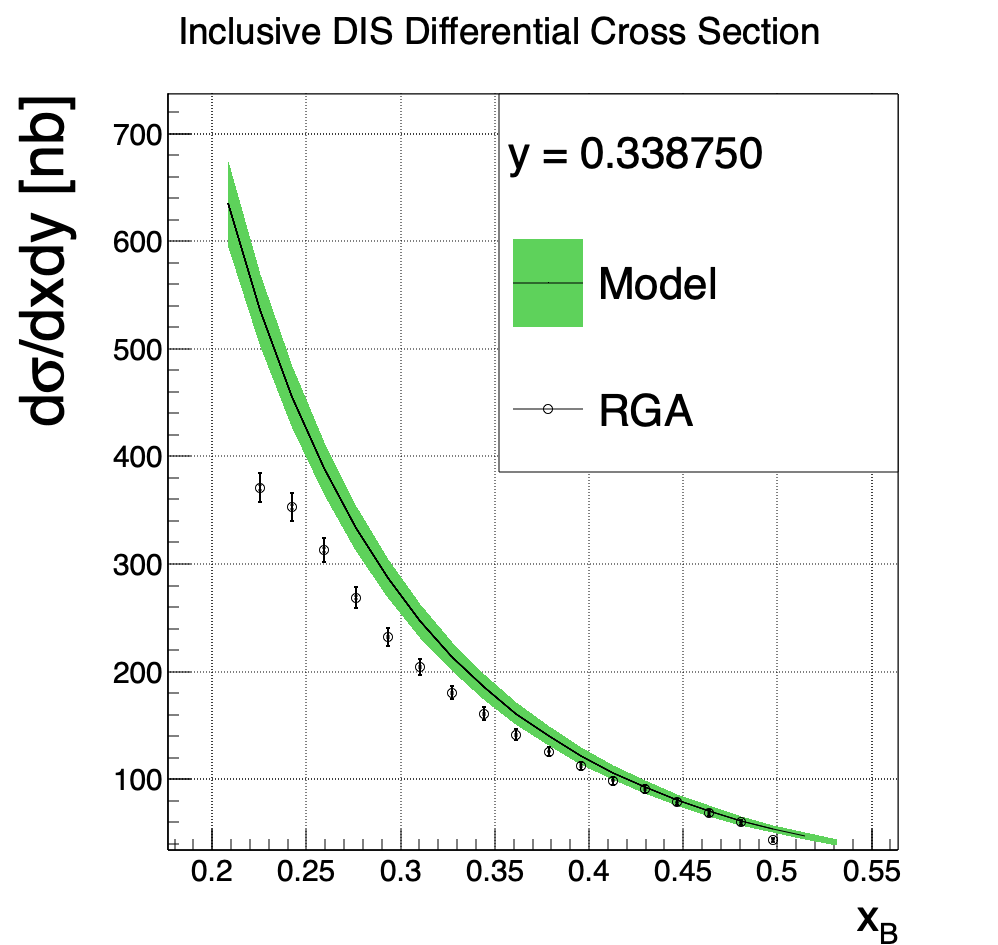
\includegraphics[width=\linewidth]{figures/rga/xsec_0.png}
		\label{fig:rga_xsec0}
	\end{subfigure}
	\begin{subfigure}[b]{0.44\textwidth}
		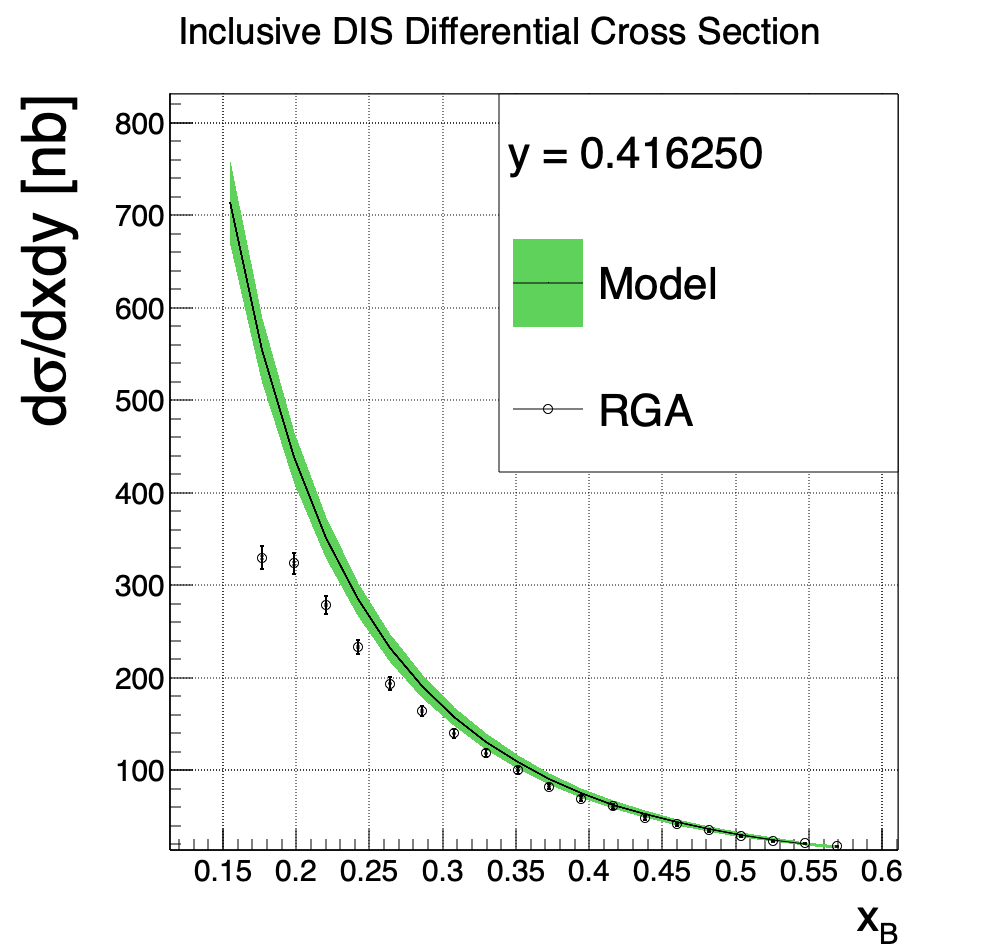
\includegraphics[width=\linewidth]{figures/rga/xsec_1.png}
		\label{fig:rga_xsec1}
	\end{subfigure}
\end{figure}
\begin{figure}[h!]
	\centering
	\begin{subfigure}[b]{0.44\linewidth}
		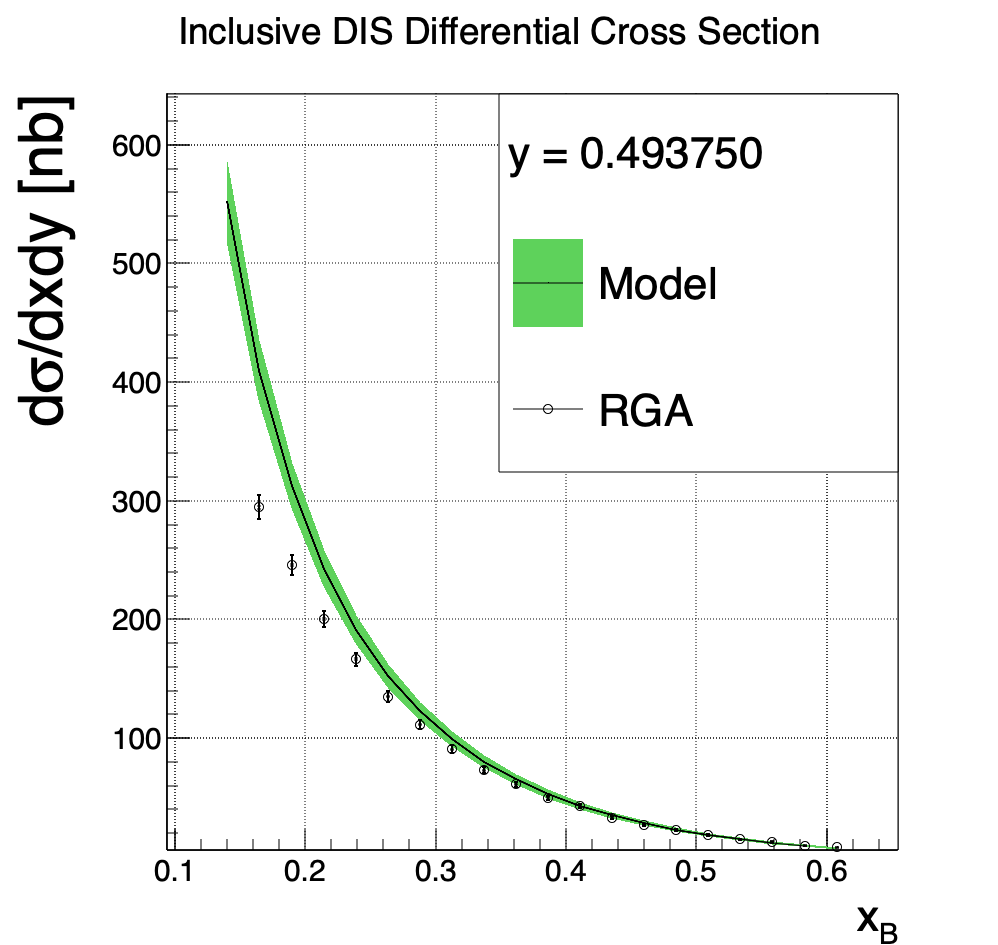
\includegraphics[width=\linewidth]{figures/rga/xsec_2.png}
		\label{fig:rga_xsec2}
	\end{subfigure}
	\begin{subfigure}[b]{0.44\textwidth}
		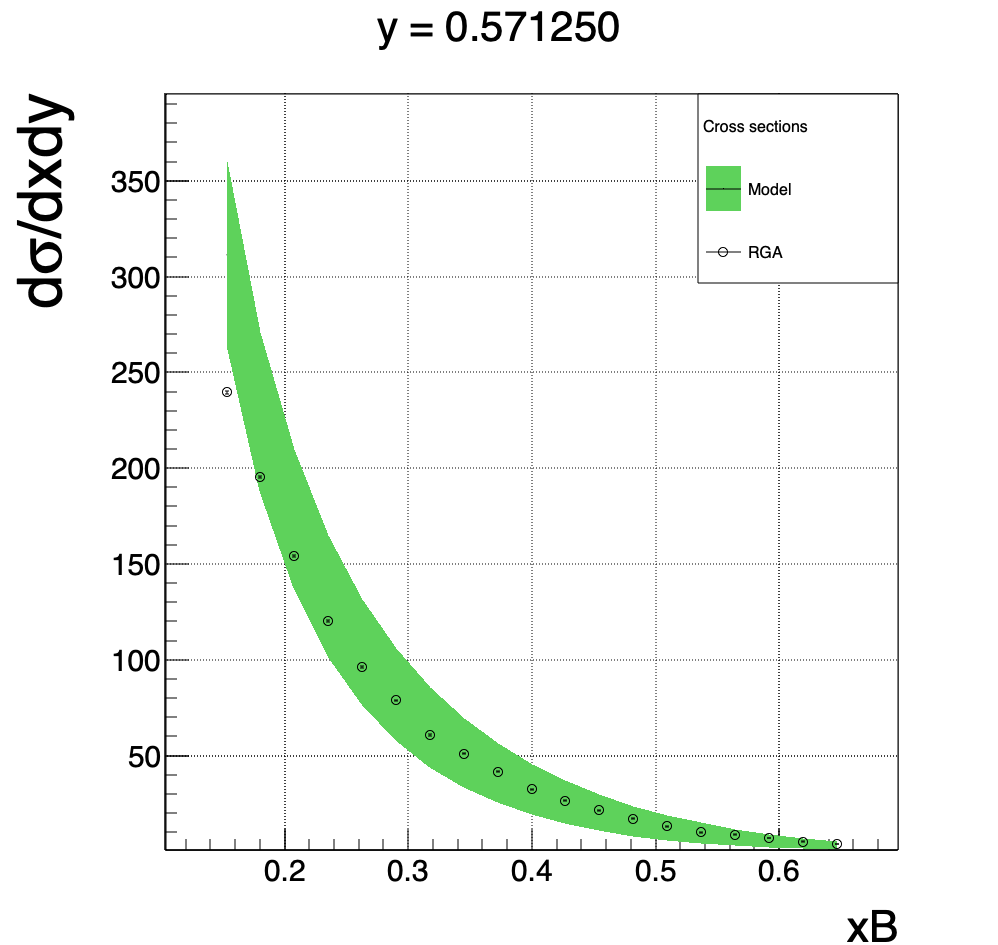
\includegraphics[width=\linewidth]{figures/rga/xsec_3.png}
		\label{fig:rga_xsec3}
	\end{subfigure}
\end{figure}
\begin{figure}[h!]
	\centering
	\begin{subfigure}[b]{0.44\linewidth}
		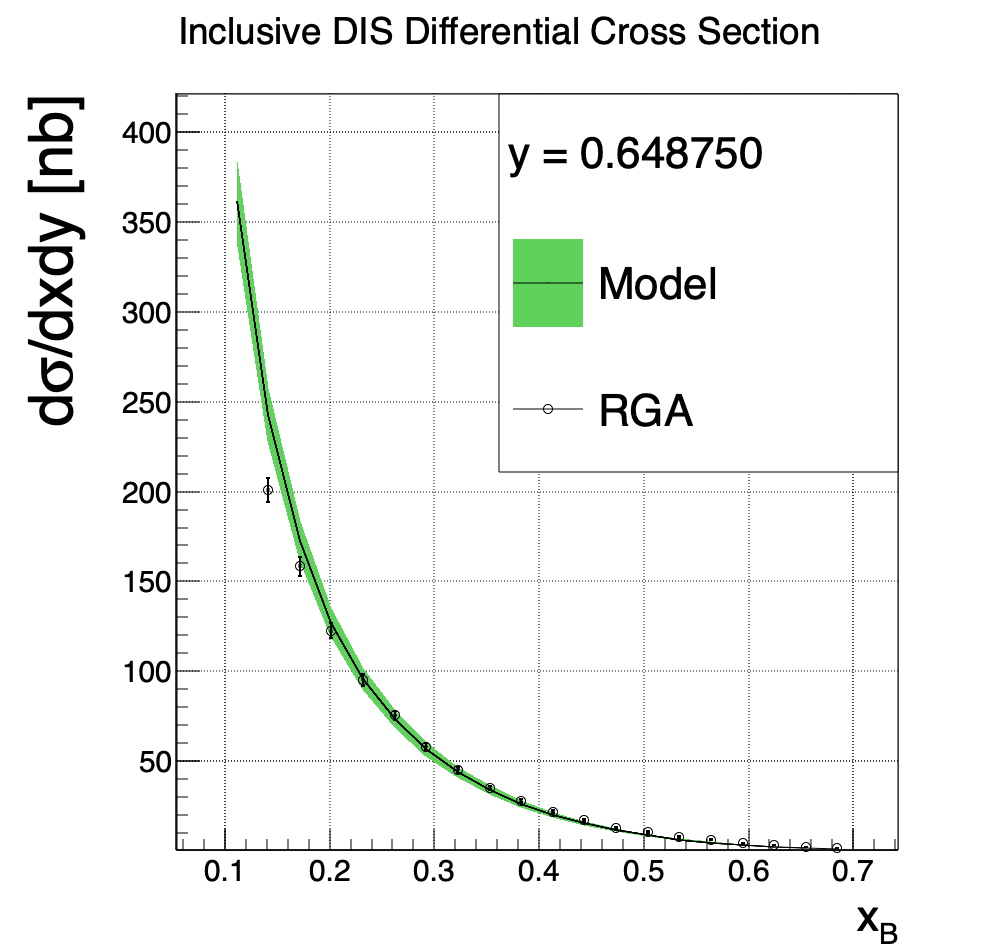
\includegraphics[width=\linewidth]{figures/rga/xsec_4.png}
		\label{fig:rga_xsec4}
	\end{subfigure}
	\begin{subfigure}[b]{0.44\textwidth}
		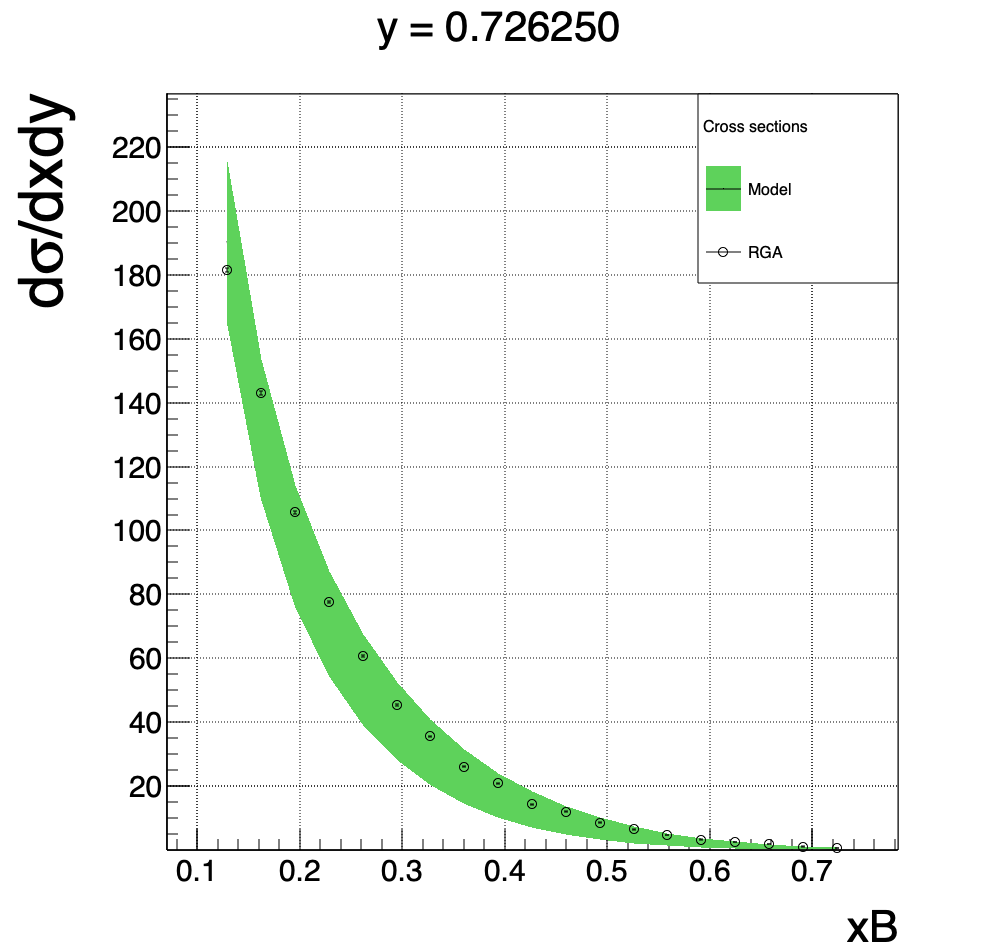
\includegraphics[width=\linewidth]{figures/rga/xsec_5.png}
		\label{fig:rga_xsec5}
	\end{subfigure}
	\caption{Plots of inclusive DIS differential cross section vs $x_B$ for various values of $y$.}
	\label{fig:rga_xsec_plots}
\end{figure}




